\chapter{常系数线性方程}

常系数线性常微分方程组是一类规模很大、地位又很重要的方程；它的解原则上可以由初等函数以及这些函数与多项式、指数的有限组合表示出来。正因如此，过去常有人以为它在理论上没有多少内容，教科书中也往往只把常系数线性方程作为一般线性方程理论的一个简单例子。事实并非如此。大量技术问题都由常系数线性方程描述，而且这些问题通常会提出新的理论要求：既要说明解的结构，也要给出适合工程计算的稳定判据、算子演算和求特解的方法。本章若干内容正是围绕这些要求展开的。

本章将讨论工程中常用的微分算子法。它把微分方程看作以 \(D=\frac{\dd}{\dd t}\) 为符号的多项式方程，特别适合用消去法处理线性方程组。本章还要研究线性方程与线性方程组解的稳定性，因为自动控制理论中经常需要判断长期行为。对于受周期外力作用的系统，复数振幅法能够迅速给出稳定特解，它在电路技术中尤其常用。因此，本章并不只处理从实际中提炼出来的个别数学问题，还会对电路理论作一个简洁而系统的介绍；电路恰好为这些数学方法提供了重要而具体的模型。

本章后半部还要研究常系数二阶线性系统的相平面。它是自治系统相空间理论的基础，而自治系统，包括一般非线性自治系统，在技术中也有广泛用途。由于这些应用背景，本书关于常系数线性方程的篇幅大于一般常微分方程教科书中的相应部分。本章材料本质上仍是初等的；只有后面的 §14 会系统使用矩阵的 Jordan 型。即使在那里，后面各节真正反复使用的也只是“互异特征值可对角化”这一较初等的事实，关于一般 Jordan 型的内容不影响后续阅读。

\setcounter{section}{6}
\setcounter{theorem}{3}

\section{常系数线性齐次方程（单根情形）}

这一节和下一节要求解 \(n\) 阶常系数线性齐次方程
\begin{equation}
 y^{(n)}+a_1y^{(n-1)}+\cdots+a_{n-1}y'+a_ny=0,
 \label{eq:ch2-7-homogeneous}
\end{equation}
其中未知函数 \(y=y(t)\) 定义在实自变量 \(t\) 的某个区间上，而
\[
 a_1,a_2,\ldots,a_n
\]
都是实常数或复常数。我们首先求出这个方程的全部复值解；当所有系数都是实数时，再从复值解中分离出全部实值解。

把最高阶导数解出，可把 \eqref{eq:ch2-7-homogeneous} 写成
\begin{equation}
 y^{(n)}
 =-a_1y^{(n-1)}-\cdots-a_{n-1}y'-a_ny.
 \label{eq:ch2-7-solved-highest}
\end{equation}
于是关于高阶方程的存在与唯一性定理可以应用于它。下面实际上只需要唯一性：方程的解将被明确构造出来，所以存在性也随之得到；唯一性则用来证明没有漏掉任何解。

在工程应用中，常系数常微分方程的算子法具有重要作用。这里先建立它的符号基础。对函数求导的运算记为
\[
 D=\frac{\dd}{\dd t},
 \qquad D^k=\frac{\dd^k}{\dd t^k}\quad(k=0,1,2,\ldots).
\]
原书使用字母 \(p\) 表示 \(d/dt\)；本稿统一把作用在函数上的算子写作 \(D\)，把对应的普通多项式写作 \(L(s)\)。这样就不必用同一字母同时表示微分运算与复变量。

\medskip
\noindent\textbf{定义 (A)：常系数微分算子.}
设
\begin{equation}
 L(s)=a_0s^n+a_1s^{n-1}+\cdots+a_{n-1}s+a_n
 \label{eq:ch2-7-polynomial}
\end{equation}
是常系数多项式，系数属于 \(\R\) 或 \(\C\)。把 \(s\) 换成微分算子 \(D\)，并令算子多项式作用在足够多次可微的函数 \(y\) 上：
\begin{equation}
 L(D)y
 =a_0D^ny+a_1D^{n-1}y+\cdots+a_{n-1}Dy+a_ny.
 \label{eq:ch2-7-operator-definition}
\end{equation}
这就是常系数线性微分算子 \(L(D)\) 的定义。若 \(L_1,L_2\) 是两个多项式，\(y_1,y_2\) 是足够光滑的函数，则由求导的线性性以及
\[
 D^kD^\ell y=D^{k+\ell}y,
\]
立即得到
\begin{align}
 L_1(D)(y_1+y_2)&=L_1(D)y_1+L_1(D)y_2,\notag\\
 \bigl(L_1(D)+L_2(D)\bigr)y&=L_1(D)y+L_2(D)y,
 \label{eq:ch2-7-operator-identities}\\
 L_1(D)\bigl(L_2(D)y\bigr)&=\bigl(L_1(D)L_2(D)\bigr)y.\notag
\end{align}
这些恒等式说明，常系数算子之间的加法与乘法可以按普通多项式进行；求导因子的先后次序并不影响结果。

原方程 \eqref{eq:ch2-7-homogeneous} 的首项系数为 \(1\)，因此可以写成
\begin{equation}
 L(D)y=0,
 \qquad
 L(s)=s^n+a_1s^{n-1}+\cdots+a_{n-1}s+a_n.
 \label{eq:ch2-7-Ly-zero}
\end{equation}

\medskip
\noindent\textbf{命题 (B).}
若 \(L(s)\) 是任意常系数多项式，则对每个复数 \(\lambda\)，
\begin{equation}
 L(D)e^{\lambda t}=L(\lambda)e^{\lambda t}.
 \label{eq:ch2-7-exponential-eigenfunction}
\end{equation}

\begin{proof}
首先有
\[
 De^{\lambda t}=\lambda e^{\lambda t},
\]
反复求导便得到
\[
 D^k e^{\lambda t}=\lambda^k e^{\lambda t},
 \qquad k=0,1,\ldots.
\]
代入算子多项式的定义，便得到
\[
 L(D)e^{\lambda t}
 =\left(\sum_{k=0}^n a_kD^{n-k}\right)e^{\lambda t}
 =\left(\sum_{k=0}^n a_k\lambda^{n-k}\right)e^{\lambda t}
 =L(\lambda)e^{\lambda t}.
\]
\end{proof}

由 \eqref{eq:ch2-7-exponential-eigenfunction}，函数 \(e^{\lambda t}\) 是齐次方程 \eqref{eq:ch2-7-Ly-zero} 的解，当且仅当
\[
 L(\lambda)=0.
\]
因此，原微分方程对应的普通多项式 \(L(s)\) 称为它的\emph{特征多项式}；它的根称为特征根。函数 \(e^{\lambda t}\) 是关于 \(D\) 的特征函数，特征根 \(\lambda\) 则是相应的特征值。这个观点与线性代数中“算子作用于特征向量后只多出一个标量因子”的说法完全一致，只是这里的向量位于函数空间中。

当特征多项式没有重根时，方程的全部解由下面的定理给出。

\begin{theorem}[单根情形的基本解组]
\label{thm:ch2-4-simple-roots}
 假设
 \begin{equation}
  L(D)y=0
  \label{eq:ch2-7-theorem4-equation}
 \end{equation}
 的特征多项式 \(L(s)\) 没有重根，并设 \(\lambda_1,\ldots,\lambda_n\) 是它的 \(n\) 个互不相同的根。令
 \begin{equation}
  y_j(t)=e^{\lambda_jt},
  \qquad j=1,\ldots,n.
  \label{eq:ch2-7-simple-fundamental-functions}
 \end{equation}
 那么对任意复常数 \(c_1,\ldots,c_n\)，函数
 \begin{equation}
  y(t)=c_1e^{\lambda_1t}+\cdots+c_ne^{\lambda_nt}
  \label{eq:ch2-7-general-complex-solution}
 \end{equation}
 都是方程 \eqref{eq:ch2-7-theorem4-equation} 的解；反过来，方程的每一个解都能唯一地写成 \eqref{eq:ch2-7-general-complex-solution} 的形式。也就是说，任意给定解都唯一确定一组积分常数 \(c_1,\ldots,c_n\)。
\end{theorem}

\begin{proof}
由命题 (B)，每个 \(e^{\lambda_jt}\) 都是齐次方程的解。齐次方程的解对线性组合封闭，所以任意复常数 \(c_1,\ldots,c_n\) 所给出的 \eqref{eq:ch2-7-general-complex-solution} 都是解。

设 \(y_*(t)\) 是方程的任意一个解。由高阶线性方程的唯一性定理，可以把它的定义区间取为整条实轴。令
\begin{equation}
 y_*(0)=y_0,\qquad
 \dot y_*(0)=y_1,\qquad\ldots,\qquad
 y_*^{(n-1)}(0)=y_{n-1}.
 \label{eq:ch2-7-initial-vector}
\end{equation}
要证明 \(y_*\) 具有 \eqref{eq:ch2-7-general-complex-solution} 的形式，只须选取 \(c_1,\ldots,c_n\)，使得由 \eqref{eq:ch2-7-general-complex-solution} 定义的新解满足同一组初始条件。

记 \(y_j^{(r)}=D^ry_j\)。把 \eqref{eq:ch2-7-general-complex-solution} 代入初始条件，得到 \(n\) 个线性方程：
\begin{equation}
 c_1y_1^{(r)}(0)+\cdots+c_ny_n^{(r)}(0)=y_r,
 \qquad r=0,1,\ldots,n-1.
 \label{eq:ch2-7-initial-linear-system}
\end{equation}
其系数矩阵为
\begin{equation}
 \begin{pmatrix}
  y_1(0)&y_2(0)&\cdots&y_n(0)\\
  y_1'(0)&y_2'(0)&\cdots&y_n'(0)\\
  \vdots&\vdots&&\vdots\\
  y_1^{(n-1)}(0)&y_2^{(n-1)}(0)&\cdots&y_n^{(n-1)}(0)
 \end{pmatrix}.
 \label{eq:ch2-7-wronskian-matrix}
\end{equation}
由于 \(D^re^{\lambda t}=\lambda^re^{\lambda t}\)，这个矩阵就是
\begin{equation}
 \begin{pmatrix}
  1&1&\cdots&1\\
  \lambda_1&\lambda_2&\cdots&\lambda_n\\
  \lambda_1^2&\lambda_2^2&\cdots&\lambda_n^2\\
  \vdots&\vdots&&\vdots\\
  \lambda_1^{n-1}&\lambda_2^{n-1}&\cdots&\lambda_n^{n-1}
 \end{pmatrix}.
 \label{eq:ch2-7-vandermonde}
\end{equation}
当 \(\lambda_1,\ldots,\lambda_n\) 两两不同时，其行列式是非零 Vandermonde 行列式。因此方程组 \eqref{eq:ch2-7-initial-linear-system} 有唯一的解 \((c_1,\ldots,c_n)\)。

原书在这里再给出一个不直接引用 Vandermonde 公式的论证，因为它可推广到重根情形。假设矩阵 \eqref{eq:ch2-7-wronskian-matrix} 的行线性相关。于是存在不全为零的常数 \(b_{n-1},b_{n-2},\ldots,b_0\)，使得依次用它们乘各行再相加后得到零行。考察所得零行的第 \(j\) 列：
\begin{equation}
 b_{n-1}y_j(0)+b_{n-2}y_j'(0)+\cdots+b_0y_j^{(n-1)}(0)=0,
 \qquad j=1,\ldots,n.
 \label{eq:ch2-7-row-relation}
\end{equation}
令
\[
 M(s)=b_0s^{n-1}+b_1s^{n-2}+\cdots+b_{n-2}s+b_{n-1}.
\]
则 \eqref{eq:ch2-7-row-relation} 等价于
\[
 M(D)e^{\lambda_jt}\big|_{t=0}=M(\lambda_j)=0,
 \qquad j=1,\ldots,n.
\]
这说明次数不超过 \(n-1\) 的多项式 \(M(s)\) 有 \(n\) 个互不相同的根 \(\lambda_1,\ldots,\lambda_n\)。除非 \(M\equiv0\)，非零多项式不可能有这么多根；但 \(b_0,\ldots,b_{n-1}\) 不全为零，所以 \(M\not\equiv0\)，矛盾。因此矩阵 \eqref{eq:ch2-7-wronskian-matrix} 非奇异。

于是可以并且唯一地选出一组常数，使构造出的解与 \(y_*\) 满足同样的初始条件。由唯一性，两者在整条实轴上相同。常数之所以唯一，也因为方程组的系数矩阵非奇异。定理得证。
\end{proof}

定理中的函数组 \eqref{eq:ch2-7-simple-fundamental-functions} 称为齐次方程的一个基本解组；它们在整个实轴上定义。解空间由这些函数张成，维数等于特征多项式的次数 \(n\)。

若特征多项式 \(L(s)\) 的系数全为实数，则复值解总体 \eqref{eq:ch2-7-general-complex-solution} 中还要分辨哪些解是实值的。下面的向量命题是处理这一点的工具。

\medskip
\noindent\textbf{命题 (C).}
把 \(n\) 个复数排成列向量
\[
 \vect{z}=
 \begin{pmatrix}
  z_1\\ \vdots\\ z_n
 \end{pmatrix}\in\C^n.
\]
复共轭按分量定义为
\[
 \overline{\vect{z}}=
 \begin{pmatrix}
  \overline z_1\\ \vdots\\ \overline z_n
 \end{pmatrix}.
\]
向量 \(\vect{z}\) 为实向量当且仅当 \(\overline{\vect{z}}=\vect{z}\)。有限个向量 \(\vect{z}_1,\ldots,\vect{z}_r\in\C^n\) 线性相关，是指存在不全为零的复常数 \(\alpha_1,\ldots,\alpha_r\)，使得
\[
 \alpha_1\vect{z}_1+\cdots+\alpha_r\vect{z}_r=\vect{0};
\]
不存在这样的常数时称它们线性无关。若 \(r=n\)，把 \(\vect{z}_j\) 作为第 \(j\) 列组成方阵，则这些列向量线性无关当且仅当该方阵的行列式不为零。

\medskip
\noindent\textbf{命题 (D).}
设 \(\vect{z}_1,\ldots,\vect{z}_n\) 是 \(\C^n\) 中 \(n\) 个线性无关的复向量，并假设这组向量在含有某个向量的同时也含有它的复共轭。对于
\begin{equation}
 \vect{z}=c_1\vect{z}_1+\cdots+c_n\vect{z}_n,
 \label{eq:ch2-7-complex-linear-combination}
\end{equation}
向量 \(\vect{z}\) 是实向量，当且仅当互为共轭的一对向量前面的系数也互为共轭，实向量前面的系数为实数。

\begin{proof}
为书写明确，把编号安排成
\[
 \overline{\vect{z}}_1=\vect{z}_2,\quad\ldots,\quad
 \overline{\vect{z}}_{2k-1}=\vect{z}_{2k},
 \qquad
 \overline{\vect{z}}_j=\vect{z}_j\quad(j=2k+1,\ldots,n).
\]
于是
\begin{align}
 \vect{z}&=c_1\vect{z}_1+c_2\vect{z}_2+\cdots+c_{2k-1}\vect{z}_{2k-1}
   +c_{2k}\vect{z}_{2k}
   +c_{2k+1}\vect{z}_{2k+1}+\cdots+c_n\vect{z}_n,\notag\\
 \overline{\vect{z}}
 &=\overline{c_1}\,\vect{z}_2+\overline{c_2}\,\vect{z}_1+\cdots
   +\overline{c_{2k-1}}\,\vect{z}_{2k}
   +\overline{c_{2k}}\,\vect{z}_{2k-1}\notag\\
 &\qquad+\overline{c_{2k+1}}\,\vect{z}_{2k+1}+\cdots
   +\overline{c_n}\,\vect{z}_n.
 \label{eq:ch2-7-conjugate-combination}
\end{align}
若
\begin{equation}
 c_1=\overline{c_2},\quad\ldots,\quad
 c_{2k-1}=\overline{c_{2k}},
 \qquad
 c_{2k+1}=\overline{c_{2k+1}},\ldots,
 c_n=\overline{c_n},
 \label{eq:ch2-7-real-coefficient-conditions}
\end{equation}
则由两式立即得到 \(\overline{\vect{z}}=\vect{z}\)。反过来，若 \(\vect{z}=\overline{\vect{z}}\)，把 \(\vect{z}\) 与 \(\overline{\vect{z}}\) 都按同一组基向量 \(\vect{z}_1,\ldots,\vect{z}_n\) 展开，比较系数，并利用这组向量的线性无关性，便得到 \eqref{eq:ch2-7-real-coefficient-conditions}。故命题成立。
\end{proof}

\medskip
\noindent\textbf{命题 (E).}
假设 \(L(s)\) 的系数全为实数。若 \(\lambda\) 是特征根，则 \(\overline\lambda\) 也是特征根；对应的指数解 \(e^{\lambda t}\) 与 \(e^{\overline\lambda t}\) 互为复共轭。若 \(\lambda\) 为实数，则 \(e^{\lambda t}\) 本身为实函数。因此，在基本解组中，每个复值解都与它的共轭解一同出现。复值线性组合 \eqref{eq:ch2-7-general-complex-solution} 为实值解，当且仅当实特征根对应的系数为实数，而每一对共轭特征根对应的系数互为共轭。

\begin{proof}
对每个特征函数，把
\[
 z_j(t)=e^{\lambda_jt},
 \quad
 z_j'(t)=\lambda_je^{\lambda_jt},
 \quad\ldots,\quad
 z_j^{(n-1)}(t)=\lambda_j^{n-1}e^{\lambda_jt}
\]
在 \(t=0\) 取值，得到向量
\[
 \vect{Z}_j=(1,\lambda_j,\ldots,\lambda_j^{n-1})^{\mathsf T}\in\C^n.
\]
再令
\[
 \vect{Z}=(y(0),y'(0),\ldots,y^{(n-1)}(0))^{\mathsf T}.
\]
线性组合 \eqref{eq:ch2-7-general-complex-solution} 给出
\[
 c_1\vect{Z}_1+\cdots+c_n\vect{Z}_n=\vect{Z}.
\]
矩阵 \eqref{eq:ch2-7-wronskian-matrix} 非奇异，所以 \(\vect{Z}_1,\ldots,\vect{Z}_n\) 线性无关。因此，解为实值当且仅当向量 \(\vect{Z}\) 为实向量；由命题 (D)，这又当且仅当共轭特征根对应的积分常数互为共轭，实特征根对应的积分常数为实数。最后，若 \(\lambda_1=\overline{\lambda_2}\) 且 \(c_1=\overline{c_2}\)，则
\[
 c_1e^{\lambda_1t}+c_2e^{\lambda_2t}
 =w+\overline w=2\operatorname{Re}w,
\]
它显然是实函数。故命题成立。
\end{proof}

\subsection*{例题}

\noindent\textbf{例 1.}
求方程
\begin{equation}
 y''' -3y''+9y'+13y=0
 \label{eq:ch2-7-example1}
\end{equation}
的全部复值解。这里
\[
 L(s)=s^3-3s^2+9s+13.
\]
直接验算可知 \(s=-1\) 是一个根，并且
\[
 L(s)=(s+1)(s^2-4s+13).
\]
二次因子给出另外两个根 \(2\pm3i\)。因此
\[
 \lambda_1=2+3i,\qquad
 \lambda_2=2-3i,\qquad
 \lambda_3=-1.
\]
由定理 4，方程的全部复值解为
\begin{equation}
 y=c_1e^{(2+3i)t}+c_2e^{(2-3i)t}+c_3e^{-t},
 \qquad c_1,c_2,c_3\in\C.
 \label{eq:ch2-7-example1-complex-general}
\end{equation}

\noindent\textbf{例 2.}
下面给出从复基本解组分离实解的一般写法。把基本解组安排成
\[
 \overline z_1=z_2,\quad\ldots,\quad
 \overline z_{2k-1}=z_{2k},
 \qquad
 \overline z_{2k+1}=z_{2k+1},\ldots,
 \overline z_n=z_n.
\]
对于一对共轭解，写
\[
 z_{2j-1}(t)=x_j(t)+iy_j(t),
 \qquad j=1,\ldots,k,
\]
其中 \(x_j,y_j\) 都是实函数。若取
\begin{equation}
 c_{2j-1}=\frac12(a_j-ib_j),
 \qquad
 c_{2j}=\frac12(a_j+ib_j),
 \qquad a_j,b_j\in\R,
 \label{eq:ch2-7-example2-real-constants}
\end{equation}
则相应的复共轭项之和为
\[
 c_{2j-1}z_{2j-1}+c_{2j}z_{2j}
 =a_jx_j+b_jy_j.
\]
所以方程的实通解可写成
\begin{equation}
 y=a_1x_1+b_1y_1+\cdots+a_kx_k+b_ky_k
 +c_{2k+1}z_{2k+1}+\cdots+c_nz_n,
 \label{eq:ch2-7-example2-real-general}
\end{equation}
其中 \(a_1,b_1,\ldots,a_k,b_k,c_{2k+1},\ldots,c_n\) 是任意实常数。

\noindent\textbf{例 3.}
仍采用上一例的共轭配对，并把复特征根写成
\[
 \lambda_{2j-1}=\mu_j+i\nu_j,
 \qquad j=1,\ldots,k.
\]
取
\begin{equation}
 c_{2j-1}=\frac12\rho_je^{i\alpha_j},
 \qquad
 c_{2j}=\frac12\rho_je^{-i\alpha_j},
 \qquad \rho_j\ge0,\quad \alpha_j\in\R.
 \label{eq:ch2-7-example3-polar-constants}
\end{equation}
那么相应的实解可以写成
\begin{equation}
 y=\rho_1e^{\mu_1t}\cos(\nu_1t+\alpha_1)+\cdots
   +\rho_ke^{\mu_kt}\cos(\nu_kt+\alpha_k)
   +c_{2k+1}e^{\lambda_{2k+1}t}+\cdots+c_ne^{\lambda_nt}.
 \label{eq:ch2-7-example3-real-solution}
\end{equation}
这里 \(\rho_j,\alpha_j\) 以及余下的实根系数都是任意实常数。这个形式说明：非零虚部 \(\nu_j\) 产生振动因子；实部 \(\mu_j>0\) 使振动振幅按指数增长，\(\mu_j<0\) 则使其按指数衰减。

\noindent\textbf{例 4.}
回到例 1，全部实值解可以写成以下两种形式：
\begin{align}
 y&=a_1e^{2t}\cos3t+b_1e^{2t}\sin3t+c_3e^{-t},
 \label{eq:ch2-7-example4-rectangular}\\
 y&=\rho_1e^{2t}\cos(3t+\alpha_1)+c_3e^{-t},
 \label{eq:ch2-7-example4-polar}
\end{align}
其中 \(a_1,b_1,c_3,\rho_1,\alpha_1\) 都是实常数，\(\rho_1\ge0\)。

\section{常系数线性齐次方程（重根情形）}

仍考虑
\begin{equation}
 L(D)y=0,
 \qquad
 L(s)=s^n+a_1s^{n-1}+\cdots+a_{n-1}s+a_n.
 \label{eq:ch2-8-equation}
\end{equation}
若特征多项式有重根，形如 \(e^{\lambda t}\) 的互异函数不可能给出 \(n\) 个不同的基本解。为寻找缺少的解，可以先看一个极限想法。设 \(\lambda_1,\lambda_2\) 是特征多项式两个不同的实根。由线性性，
\begin{equation}
 \frac{e^{\lambda_1t}-e^{\lambda_2t}}{\lambda_1-\lambda_2}
 \label{eq:ch2-8-divided-difference}
\end{equation}
也是方程的解。如果连续改变多项式系数，使 \(\lambda_2\to\lambda_1\)，这个解的形式极限是
\[
 te^{\lambda_1t}.
\]
因此很自然地猜测：当 \(\lambda_1\) 是二重根时，除 \(e^{\lambda_1t}\) 外，\(te^{\lambda_1t}\) 也应当是解。进一步，若 \(\lambda\) 是 \(k\) 重根，则应当有
\[
 e^{\lambda t},\quad te^{\lambda t},\quad\ldots,\quad
 t^{k-1}e^{\lambda t}.
\]
把这一猜测推广到所有重根，便得到下面定理。

\begin{theorem}[重根情形的基本解组]
\label{thm:ch2-5-repeated-roots}
 设 \eqref{eq:ch2-8-equation} 是 \(n\) 阶常系数线性齐次方程。设
 \[
  \lambda_1,\ldots,\lambda_m
 \]
 是特征多项式 \(L(s)\) 的全部两两不同的根，而 \(\lambda_j\) 的重数为 \(k_j\)，于是
 \[
  k_1+\cdots+k_m=n.
 \]
 把函数组按重根顺序排成
 \begin{equation}
 \left\{
 \begin{aligned}
  &e^{\lambda_1t},\,te^{\lambda_1t},\,\ldots,\,
   t^{k_1-1}e^{\lambda_1t},\\
  &e^{\lambda_2t},\,te^{\lambda_2t},\,\ldots,\,
   t^{k_2-1}e^{\lambda_2t},\\
  &\hspace{2.2cm}\vdots\\
  &e^{\lambda_mt},\,te^{\lambda_mt},\,\ldots,\,
   t^{k_m-1}e^{\lambda_mt}.
 \end{aligned}
 \right.
 \label{eq:ch2-8-fundamental-system}
 \end{equation}
 那么组 \eqref{eq:ch2-8-fundamental-system} 中的每个函数都是方程的解；因此对任意复常数 \(c_1,\ldots,c_n\)，其线性组合
 \begin{equation}
  y=c_1y_1+\cdots+c_ny_n
  \label{eq:ch2-8-general-solution}
 \end{equation}
 也是解。反过来，方程的每个解都能通过适当选取常数由 \eqref{eq:ch2-8-general-solution} 得到，而且对于同一个解，这些常数唯一确定。
\end{theorem}

在证明定理之前，先建立两个工具。

\medskip
\noindent\textbf{命题 (A)：平移公式.}
设 \(L(s)\) 是任意多项式，\(\lambda\in\C\)，而 \(f\) 是足够多次可微的函数。则
\begin{equation}
 L(D)\bigl(e^{\lambda t}f(t)\bigr)
 =e^{\lambda t}L(D+\lambda)f(t).
 \label{eq:ch2-8-shift-formula}
\end{equation}
右端的 \(L(D+\lambda)\) 表示把多项式 \(L(s)\) 中的自变量 \(s\) 形式地替换成 \(D+\lambda\)。

\begin{proof}
先看 \(L(s)=s\)：
\[
 D(e^{\lambda t}f)
 =\lambda e^{\lambda t}f+e^{\lambda t}Df
 =e^{\lambda t}(D+\lambda)f.
\]
对 \(L(s)=as+b\)，由线性性，
\[
 (aD+b)(e^{\lambda t}f)
 =ae^{\lambda t}(D+\lambda)f+be^{\lambda t}f
 =e^{\lambda t}\bigl(a(D+\lambda)+b\bigr)f.
\]
一般情形可按多项式次数归纳。假设公式对所有次数小于 \(n\) 的多项式成立，并把 \(n\) 次多项式分解为
\[
 L(s)=L_1(s)L_2(s),
\]
其中 \(L_1\) 是一次，\(L_2\) 是 \(n-1\) 次。利用算子多项式的乘积法则以及归纳假设，
\begin{align*}
 L_1(D)\bigl(L_2(D)(e^{\lambda t}f)\bigr)
 &=L_1(D)\bigl(e^{\lambda t}L_2(D+\lambda)f\bigr)\\
 &=e^{\lambda t}L_1(D+\lambda)L_2(D+\lambda)f\\
 &=e^{\lambda t}L(D+\lambda)f.
\end{align*}
因此公式 \eqref{eq:ch2-8-shift-formula} 对一切多项式成立。
\end{proof}

\medskip
\noindent\textbf{命题 (B)：重根的算子判据.}
令
\begin{equation}
 \omega_r(t)=L(D)\bigl(t^re^{\lambda t}\bigr),
 \qquad r=0,1,\ldots.
 \label{eq:ch2-8-omega}
\end{equation}
若 \(\lambda\) 是 \(L(s)\) 的 \(k\) 重根，则
\[
 \omega_0(t)=\cdots=\omega_{k-1}(t)\equiv0.
\]
反过来，若对某个 \(t=t_0\) 有
\begin{equation}
 \omega_0(t_0)=\omega_1(t_0)=\cdots=\omega_{k-1}(t_0)=0,
 \label{eq:ch2-8-multiplicity-condition}
\end{equation}
则 \(\lambda\) 是 \(L(s)\) 的根，而且重数至少为 \(k\)。

\begin{proof}
由平移公式，
\begin{equation}
 \omega_r(t)
 =e^{\lambda t}L(D+\lambda)t^r.
 \label{eq:ch2-8-omega-shift}
\end{equation}
先设 \(\lambda\) 是 \(k\) 重根，于是
\[
 L(s)=M(s)(s-\lambda)^k,
 \qquad M(\lambda)\ne0.
\]
把 \(s\) 换成 \(D+\lambda\)，得到
\[
 L(D+\lambda)=M(D+\lambda)D^k.
\]
当 \(r=0,1,\ldots,k-1\) 时，\(D^k t^r=0\)，所以 \(\omega_r\equiv0\)。

反过来，假设 \eqref{eq:ch2-8-multiplicity-condition} 成立。把 \(L(D+\lambda)\) 按 \(D\) 的幂展开为
\begin{equation}
 L(D+\lambda)=b_0+b_1D+\cdots+b_nD^n.
 \label{eq:ch2-8-expanded-shift}
\end{equation}
由 \eqref{eq:ch2-8-omega-shift}，在 \(t=t_0\) 处
\[
 \omega_0(t_0)=e^{\lambda t_0}b_0.
\]
由 \(\omega_0(t_0)=0\)，得 \(b_0=0\)，即 \(L(\lambda)=0\)。

再假设已经证明
\[
 b_0=b_1=\cdots=b_{r-1}=0
\quad(0\le r\le k-1).
\]
由于 \(D^\ell t^r|_{t=t_0}=0\) 对 \(0\le\ell<r\) 成立，而 \(D^rt^r=r!\)，所以
\[
 \omega_r(t_0)
 =e^{\lambda t_0}L(D+\lambda)t^r\big|_{t=t_0}
 =e^{\lambda t_0}r!b_r.
\]
条件 \(\omega_r(t_0)=0\) 给出 \(b_r=0\)。逐步归纳得
\[
 b_0=b_1=\cdots=b_{k-1}=0.
\]
因此 \(L(D+\lambda)\) 能被 \(D^k\) 整除；把 \(D\) 换回 \(s-\lambda\)，便知 \(L(s)\) 能被 \((s-\lambda)^k\) 整除。所以 \(\lambda\) 至少是 \(k\) 重根。
\end{proof}

\begin{proof}[定理 5 的证明]
命题 (B) 已经证明函数组 \eqref{eq:ch2-8-fundamental-system} 中每个函数都是方程的解，因此它们的任意线性组合也是解。还需证明任意解都能由这组函数表示，并且系数唯一。

设 \(y_*(t)\) 是方程在某个区间上的任意解，取该区间内一点 \(t_0\)。记
\[
 y_*^{(r)}(t_0)=y_r,
 \qquad r=0,1,\ldots,n-1.
\]
我们寻找常数 \(c_1,\ldots,c_n\)，使线性组合 \eqref{eq:ch2-8-general-solution} 满足同一组初始条件。代入后得到
\begin{equation}
 c_1y_1^{(r)}(t_0)+\cdots+c_ny_n^{(r)}(t_0)=y_r,
 \qquad r=0,1,\ldots,n-1.
 \label{eq:ch2-8-initial-system}
\end{equation}
只要系数矩阵
\begin{equation}
 \begin{pmatrix}
  y_1(t_0)&y_2(t_0)&\cdots&y_n(t_0)\\
  y_1'(t_0)&y_2'(t_0)&\cdots&y_n'(t_0)\\
  \vdots&\vdots&&\vdots\\
  y_1^{(n-1)}(t_0)&y_2^{(n-1)}(t_0)&\cdots&
  y_n^{(n-1)}(t_0)
 \end{pmatrix}
 \label{eq:ch2-8-initial-matrix}
\end{equation}
非奇异，方程组就有唯一解。由唯一性定理，所得解与 \(y_*\) 相同；同时常数也唯一。

假设矩阵 \eqref{eq:ch2-8-initial-matrix} 奇异，则其各行线性相关。存在不全为零的常数 \(b_{n-1},b_{n-2},\ldots,b_0\)，使得依次乘各行并相加得到零行。考察第 \(j\) 列，得到
\begin{equation}
 b_{n-1}y_j(t_0)+b_{n-2}y_j'(t_0)+\cdots
 +b_0y_j^{(n-1)}(t_0)=0,
 \qquad j=1,\ldots,n.
 \label{eq:ch2-8-matrix-row-relation}
\end{equation}
令
\[
 M(s)=b_0s^{n-1}+b_1s^{n-2}+\cdots+b_{n-2}s+b_{n-1}.
\]
则上式就是
\begin{equation}
 M(D)y_j(t)\big|_{t=t_0}=0,
 \qquad j=1,\ldots,n.
 \label{eq:ch2-8-M-annihilates-fundamental}
\end{equation}
对于重根 \(\lambda_1\)，前 \(k_1\) 个基本解是
\(e^{\lambda_1t},te^{\lambda_1t},\ldots,t^{k_1-1}e^{\lambda_1t}\)。
所以 \eqref{eq:ch2-8-M-annihilates-fundamental} 对这些函数都成立；由命题 (B)，\(\lambda_1\) 至少是 \(M(s)\) 的 \(k_1\) 重根。对 \(\lambda_2\) 得到至少 \(k_2\) 重，依此类推。

于是次数不超过 \(n-1\) 的多项式 \(M(s)\) 至少有
\[
 k_1+\cdots+k_m=n
\]
个根，重根按重数计算，这只能迫使 \(M\equiv0\)，与 \(b_0,\ldots,b_{n-1}\) 不全为零矛盾。因此矩阵 \eqref{eq:ch2-8-initial-matrix} 非奇异，定理得证。
\end{proof}

\medskip
\noindent\textbf{命题 (C).}
方程 \eqref{eq:ch2-8-equation} 的每个解都能唯一地写成
\begin{equation}
 y(t)=f_1(t)e^{\lambda_1t}+\cdots+f_m(t)e^{\lambda_mt},
 \label{eq:ch2-8-polynomial-exponential-form}
\end{equation}
其中 \(f_j(t)\) 是次数不超过 \(k_j-1\) 的多项式。由于这些多项式的系数就是定理 5 中唯一的积分常数，它们也由解 \(y\) 唯一确定。

\medskip
\noindent\textbf{命题 (D).}
假设特征多项式 \(L(s)\) 的系数全为实数，\(\lambda\) 是它的 \(k\) 重根。对
\(r=0,1,\ldots,k-1\)，函数 \(t^re^{\lambda t}\) 是方程的解。若 \(\lambda\) 为实数，则这些函数都是实的；若 \(\lambda\) 为复数，则 \(\overline\lambda\) 也是 \(k\) 重根，并且 \(t^re^{\overline\lambda t}\) 与 \(t^re^{\lambda t}\) 互为复共轭。因此，为了让复值线性组合成为实解，实根项所带的系数必须为实数，每对共轭根项所带的系数必须互为共轭。

其证明与 §7 命题 (E) 完全相同：把基本解及其直到 \(n-1\) 阶导数在一点的值组成实向量，再应用命题 (D) 的实向量判据即可。

\subsection*{例题}

\noindent\textbf{例 1.}
解方程
\begin{equation}
 y^{(5)}+3y^{(4)}+3y'''+y''=0.
 \label{eq:ch2-8-example1}
\end{equation}
特征多项式为
\[
 L(s)=s^5+3s^4+3s^3+s^2=s^2(s+1)^3.
\]
所以
\[
 \lambda_1=0\quad(k_1=2),
 \qquad
 \lambda_2=-1\quad(k_2=3).
\]
基本解组为
\[
 1,\quad t,\quad e^{-t},\quad te^{-t},\quad t^2e^{-t}.
\]
故通解为
\begin{equation}
 y=(c_1+c_2t)+(c_3+c_4t+c_5t^2)e^{-t}.
 \label{eq:ch2-8-example1-general}
\end{equation}

\noindent\textbf{例 2.}
解方程
\begin{equation}
 y^{(4)}+2y''+y=0.
 \label{eq:ch2-8-example2}
\end{equation}
特征多项式为
\[
 L(s)=(s^2+1)^2=(s-i)^2(s+i)^2.
\]
两个二重根为 \(\lambda_1=i,\lambda_2=-i\)。因此复通解为
\begin{equation}
 y=(c_1+c_2t)e^{it}+(c_3+c_4t)e^{-it}.
 \label{eq:ch2-8-example2-general}
\end{equation}

\noindent\textbf{例 3.}
在重根情形中，分离实解的规则与 §7 例 2 相同：把每一对共轭基本解
\[
 t^re^{\lambda t},\qquad t^re^{\overline\lambda t}
\]
换成其中一个的实部和虚部。所得实基本解组具有这样的性质：任意实解都是它们的实系数线性组合。

\noindent\textbf{例 4.}
若
\[
 \lambda=\mu+i\nu,
 \qquad \nu\ne0,
\]
而一对共轭项前面的系数取为
\[
 c=\frac12\rho e^{i\alpha},
 \qquad
 \overline c=\frac12\rho e^{-i\alpha},
\]
那么这一对共轭项之和为
\begin{equation}
 ct^re^{(\mu+i\nu)t}+\overline c\,t^re^{(\mu-i\nu)t}
 =\rho t^re^{\mu t}\cos(\nu t+\alpha).
 \label{eq:ch2-8-real-repeated-term}
\end{equation}
于是可以用两对任意实常数 \((\rho_j,\alpha_j)\) 代替复共轭常数对。

与 §7 例 3 一样，根的非零虚部产生振动因子，根的实部决定指数增长或衰减。重数 \(r+1\) 额外引入因子 \(t^r\)。它可能使短时间内的增长看起来更强，但若 \(\mu<0\)，指数衰减 \(e^{\mu t}\) 最终仍压过多项式因子，任何固定重数的解在 \(t\to+\infty\) 时都趋于零。

\noindent\textbf{例 5.}
由例 3 和例 4，例 2 的全部实解可以写成
\begin{align}
 y&=(a_1+a_2t)\cos t+(b_1+b_2t)\sin t,
 \label{eq:ch2-8-example2-real-rectangular}\\
 y&=\rho_1\cos(t+\alpha_1)+t\rho_2\cos(t+\alpha_2).
 \label{eq:ch2-8-example2-real-polar}
\end{align}
第二式中的第二项含因子 \(t\)，表示重根带来的线性多项式包络；这层含义由第一式直接可见。

\section{稳定多项式}

仍设
\begin{equation}
 L(D)y=0
 \label{eq:ch2-9-equation}
\end{equation}
是常系数线性齐次方程。当 \(t\to+\infty\) 时，它的解是趋于零、保持有界，还是无限增长，是常微分方程应用中最重要的问题之一。§7 例 3 和 §8 例 4 已经说明，长期行为由特征根实部的符号控制。现在把这一联系写成一般判据。

\medskip
\noindent\textbf{定义 (A).}
若多项式 \(L(s)\) 的所有根都有严格负实部，也就是说所有根都位于复平面虚轴的左侧，则称 \(L(s)\) 为\emph{稳定多项式}。

设特征根为
\[
 \lambda_j=\mu_j+i\nu_j,
 \qquad j=1,\ldots,m,
\]
其中同一个根只列一次，但后面的估计会同时利用它的重数。由有限个根和严格不等式 \(\mu_j<0\)，总存在正数 \(\alpha\)，使得
\begin{equation}
 \mu_j<-\alpha,
 \qquad j=1,\ldots,m.
 \label{eq:ch2-9-negative-spectral-gap}
\end{equation}
我们证明此时存在正数 \(M\)，使得方程 \eqref{eq:ch2-9-equation} 的每个解 \(y(t)\) 都满足
\begin{equation}
 |y(t)|<Me^{-\alpha t},
 \qquad t\ge0.
 \label{eq:ch2-9-exponential-estimate}
\end{equation}
这个估计不仅说明所有解趋于零，还给出统一的指数衰减速度。

\begin{proof}
先对 §8 基本解组中的任意一个函数
\[
 y_j(t)=t^re^{\lambda_jt}
\]
证明相应估计。由 \eqref{eq:ch2-9-negative-spectral-gap}，
\[
 \left|\frac{y_j(t)}{e^{-\alpha t}}\right|
 =t^re^{(\mu_j+\alpha)t}.
\]
因为 \(\mu_j+\alpha<0\)，函数 \(t^re^{(\mu_j+\alpha)t}\) 当 \(t\to+\infty\) 时趋于零，所以它在 \([0,+\infty)\) 上有界。于是存在 \(M_j>0\)，使
\[
 \left|\frac{y_j(t)}{e^{-\alpha t}}\right|<M_j,
 \qquad t\ge0,
\]
等价地，
\begin{equation}
 |y_j(t)|<M_je^{-\alpha t},
 \qquad t\ge0.
 \label{eq:ch2-9-basis-estimate}
\end{equation}

任意解可以写成
\[
 y(t)=c_1y_1(t)+\cdots+c_ny_n(t).
\]
于是当 \(t\ge0\) 时，
\begin{align*}
 |y(t)|
 &\le |c_1||y_1(t)|+\cdots+|c_n||y_n(t)|\\
 &\le \bigl(|c_1|M_1+\cdots+|c_n|M_n\bigr)e^{-\alpha t}.
\end{align*}
取
\[
 M=|c_1|M_1+\cdots+|c_n|M_n
\]
即可。若解不是零解，还可以把严格不等式改成不超过某个常数；这里取更大的 \(M\) 不影响证明。
\end{proof}

反过来，如果 \(L(s)\) 至少有一个根 \(\lambda_j\) 的实部 \(\mu_j>0\)，则对应的解 \(e^{\lambda_jt}\) 的模为 \(e^{\mu_jt}\)，当 \(t\to+\infty\) 时无限增长。因此，所有根实部严格为负是“每条解都按指数速度趋于零”的充分条件；对本节的常系数齐次方程，它也是必要条件。

找出便于实际使用的稳定性代数判据，长期吸引了许多数学家的研究。二次多项式可以直接由求根公式判断；任意次多项式的稳定性则由 Routh 和 Hurwitz 以略有不同的形式解决。Routh--Hurwitz 条件在实际计算中并不总是方便，因此人们不断寻求新的等价形式。下面先给出二次判据、实系数稳定性的必要条件，再证明三次情形的 Routh--Hurwitz 判据，最后陈述一般次数的 Hurwitz 判据。

\medskip
\noindent\textbf{命题 (B).}
设
\[
 L(s)=s^2+as+b,
 \qquad a,b\in\R.
\]
则 \(L(s)\) 稳定，当且仅当
\[
 a>0,\qquad b>0.
\]

\begin{proof}
两个根的和为 \(-a\)，乘积为 \(b\)。若两个根实部都为负，则根的乘积为正，所以 \(b>0\)；根的实部之和为负，所以 \(a>0\)。反过来，若 \(a>0,b>0\)，由二次方程求根公式，根或者是一对负实部的共轭复数，或者是两个和为负、乘积为正的实根；后者只能都是负实根。故稳定。
\end{proof}

\medskip
\noindent\textbf{命题 (C).}
若实系数多项式
\[
 L(s)=s^n+a_1s^{n-1}+\cdots+a_n
\]
稳定，则它的所有系数 \(a_1,\ldots,a_n\) 都为正。

\begin{proof}
把实系数多项式分解为实的一次因子 \(s+c\) 与实二次因子 \(s^2+as+b\) 的乘积。若某个一次因子本身不是稳定多项式，乘积中就会有一个根不具严格负实部，与整体稳定矛盾。因此每个一次因子稳定，故 \(c>0\)。同理，每个二次因子稳定；由命题 (B)，相应的 \(a>0,b>0\)。所有因子系数为正，逐次相乘时各项系数也都为正。所以原多项式的所有系数为正。
\end{proof}

\begin{theorem}[三次多项式的稳定判据]
\label{thm:ch2-6-cubic-stability}
 设实系数三次多项式
 \[
  L(s)=a_0s^3+a_1s^2+a_2s+a_3,
  \qquad a_0>0.
 \]
 则 \(L(s)\) 稳定，当且仅当
 \[
  a_1>0,\quad a_2>0,\quad a_3>0,
  \qquad
  a_1a_2>a_0a_3.
 \]
\end{theorem}

\begin{proof}
因 \(a_0>0\)，可除以 \(a_0\)，化为首项系数为 \(1\) 的多项式
\begin{equation}
 L(s)=s^3+as^2+bs+c.
 \label{eq:ch2-9-monic-cubic}
\end{equation}
由命题 (C)，若它稳定，必有 \(a,b,c>0\)。在这个前提下还要证明：稳定当且仅当
\begin{equation}
 ab>c.
 \label{eq:ch2-9-cubic-inequality}
\end{equation}
证明用到一件基本事实：多项式的根连续依赖于它的系数。

先判断何时会有纯虚根。这里把 \(s=0\) 也看作落在虚轴上的退化纯虚根。若 \(s=0\) 是根，则 \(c=0\)，但已假设 \(c>0\)，故不会发生。把多项式整理为
\begin{equation}
 L(s)=(s+a)(s^2+b)-ab+c.
 \label{eq:ch2-9-cubic-decomposition}
\end{equation}
设 \(s=i\omega,\omega\ne0\)，是 \(L\) 的根。则
\[
 L(i\omega)=(i\omega+a)(-\omega^2+b)-ab+c.
\]
如果 \(-\omega^2+b\ne0\)，那么 \((i\omega+a)(-\omega^2+b)\) 的虚部等于
\(\omega(b-\omega^2)\ne0\)，它不可能与实数 \(-ab+c\) 相加为零。因此必须有
\[
 b-\omega^2=0,
\]
并且
\[
 L(i\omega)=-ab+c=0.
\]
反过来，若 \(ab=c\)，由 \(b>0\) 可取 \(\omega=\sqrt b\)，上面的计算给出 \(L(\pm i\sqrt b)=0\)。因此，具有正系数 \(a,b,c\) 的三次多项式有纯虚根，当且仅当
\[
 ab=c.
\]
当系数连续改变时，根只能连续移动；若根从虚轴左侧移到右侧，途中必与虚轴相交。因此等号 \(ab=c\) 正是稳定域与不稳定域之间的边界。

若 \(ab<c\)，先连续改变正数 \(a,b\)，使它们趋于零，同时保持
\begin{equation}
 ab<c.
 \label{eq:ch2-9-bad-region}
 \end{equation}
这个过程中不能穿过边界 \(ab=c\)，所以稳定性状态不变。当 \(a=b=0\) 时，
\[
 L(s)=s^3+c.
\]
它的三个根为
\[
 -c^{1/3},\qquad
 c^{1/3}\left(\cos\frac{\pi}{3}\pm i\sin\frac{\pi}{3}\right),
\]
其中后两个根的实部为正，所以此多项式不稳定。由根对系数的连续依赖，正数 \(a,b\) 充分小时仍不稳定；因而整个 \(ab<c\) 的区域都不稳定。

若 \(ab=c\)，上面已经看到存在纯虚根，也不稳定。于是稳定必须有充分条件 \(ab>c\)。

最后假设 \(ab>c\)。让 \(c\) 连续减小并仍保持为正，直到 \(c\to0\)，过程中不穿过临界等式 \(ab=c\)。当 \(c=0\) 时，
\begin{equation}
 L(s)=s(s^2+as+b),
 \label{eq:ch2-9-boundary-cubic}
\end{equation}
有一个零根，另外两个根满足二次稳定条件 \(a>0,b>0\)，所以具有负实部。对足够小的正 \(c\)，后两个根的实部仍为负；零根则连续变为一个很小的实根。三个根之积等于 \(-c<0\)，而另外两个根的乘积为正，所以这个接近零的根必须是负实根。故在 \(ab>c\) 时三个根都有负实部，多项式稳定。定理得证。
\end{proof}

为了陈述任意次数的稳定性判据，先引入主子式。设
\[
 \mat{P}=(p_{ij})_{i,j=1}^n
\]
是 \(n\) 阶方阵。把前 \(k\) 行和前 \(k\) 列交叉处元素组成的 \(k\) 阶方阵的行列式记为
\[
 \Delta_k(\mat{P})=
 \det
 \begin{pmatrix}
  p_{11}&\cdots&p_{1k}\\
  \vdots&\ddots&\vdots\\
  p_{k1}&\cdots&p_{kk}
 \end{pmatrix},
 \qquad k=1,\ldots,n.
\]
这些数称为 \(\mat{P}\) 的\emph{顺序主子式}（也作前导主子式）。

\begin{theorem}[Hurwitz 稳定性判据]
\label{thm:ch2-7-hurwitz}
 设
 \begin{equation}
  L(s)=a_0s^n+a_1s^{n-1}+\cdots+a_n,
  \qquad a_0>0,
  \label{eq:ch2-9-hurwitz-polynomial}
 \end{equation}
 是 \(n\) 次实系数多项式。构造 \(n\) 阶 Hurwitz 矩阵
 \begin{equation}
  \mat{Q}=
  \begin{pmatrix}
   a_1&a_3&a_5&\cdots&0\\
   a_0&a_2&a_4&\cdots&0\\
   0&a_1&a_3&\cdots&0\\
   \vdots&\vdots&\vdots&\ddots&\vdots\\
   0&\cdots&a_{n-2}&a_n
  \end{pmatrix},
  \label{eq:ch2-9-hurwitz-matrix}
 \end{equation}
 其中当 \(r<0\) 或 \(r>n\) 时约定 \(a_r=0\)。则 \(L(s)\) 稳定，当且仅当
 \[
  \Delta_k(\mat{Q})>0,
  \qquad k=1,\ldots,n.
 \]
\end{theorem}

原书在正文中不展开定理 7 的证明，而是引用切塔也夫《运动稳定性》中的证明。本稿保持这一编排：定理 7 的完整补证不放在本节正文的末尾，而由本章独立的 Hurwitz 补证文件承担。下面只说明如何避免排写矩阵 \(\mat{Q}\) 时出错。矩阵 \(\mat{Q}\) 的第 \(k\) 列从主对角线元素 \(a_k\) 开始，向上依次为
\[
 \cdots,\ a_{k+2},\ a_{k+1},\ a_k,\ a_{k-1},\ a_{k-2},\ \cdots,
\]
而下标超出 \(0,\ldots,n\) 的系数按零处理。

\subsection*{例题}

\noindent\textbf{例 1.}
从定理 7 推出定理 6。当 \(n=3\) 时，
\[
 \mat{Q}=
 \begin{pmatrix}
  a_1&a_3&0\\
  a_0&a_2&0\\
  0&a_1&a_3
 \end{pmatrix}.
\]
其顺序主子式为
\[
 \Delta_1(\mat{Q})=a_1,
 \quad
 \Delta_2(\mat{Q})=a_1a_2-a_0a_3,
 \quad
 \Delta_3(\mat{Q})=a_3\Delta_2(\mat{Q}).
\]
因此
\[
 \Delta_1>0,\quad \Delta_2>0,\quad \Delta_3>0
\]
与 \(a_0>0\) 合在一起，等价于
\[
 a_0>0,\quad
 a_1>0,\quad
 a_3>0,\quad
 a_1a_2>a_0a_3.
\]
由于 \(a_1>0\) 且 \(a_1a_2>a_0a_3>0\)，还可以推出 \(a_2>0\)。于是恰为定理 6 的条件。

\noindent\textbf{例 2.}
当 \(n=4\) 时，
\[
 \mat{Q}=
 \begin{pmatrix}
  a_1&a_3&0&0\\
  a_0&a_2&a_4&0\\
  0&a_1&a_3&0\\
  0&a_0&a_2&a_4
 \end{pmatrix}.
\]
顺序主子式为
\begin{align*}
 \Delta_1(\mat{Q})&=a_1,\\
 \Delta_2(\mat{Q})&=a_1a_2-a_0a_3,\\
 \Delta_3(\mat{Q})&=a_1a_2a_3-a_0a_3^2-a_1^2a_4,\\
 \Delta_4(\mat{Q})&=a_4\Delta_3(\mat{Q}).
\end{align*}
这些量全为正，再与 \(a_0>0\) 合在一起，等价于
\[
 a_0>0,\quad a_1>0,\quad a_2>0,\quad a_3>0,\quad a_4>0,
\]
以及
\[
 \Delta_3(\mat{Q})=a_1a_2a_3-a_0a_3^2-a_1^2a_4>0.
\]
最后一个严格不等式不能用“系数全正”代替；它正体现了四次情形中根分布对系数组合的限制。

\section{常系数线性非齐次方程}

本节讨论含有自由项的常系数线性方程
\begin{equation}
 L(D)y=F(t),
 \label{eq:ch2-10-nonhomogeneous}
\end{equation}
其中自由项属于所谓拟多项式。工程中常见的多项式、指数函数、正弦与余弦以及它们的有限乘积，都可以纳入这一框架。

\medskip
\noindent\textbf{定义 (A).}
若函数可以写成
\begin{equation}
 F(t)=f_1(t)e^{\lambda_1t}+f_2(t)e^{\lambda_2t}
   +\cdots+f_m(t)e^{\lambda_mt},
 \label{eq:ch2-10-quasipolynomial}
\end{equation}
其中 \(\lambda_1,\ldots,\lambda_m\) 是复数，\(f_1(t),\ldots,f_m(t)\) 是多项式，则称 \(F(t)\) 为\emph{拟多项式}。

由 §8 命题 (C)，常系数线性齐次方程的每个解都是拟多项式。反过来也能证明：每一个拟多项式都满足某一个常系数线性齐次方程，因而都属于某一类有限维解空间。不过本节只需要拟多项式的几个封闭性质。

若 \eqref{eq:ch2-10-quasipolynomial} 中有两个指数相同，例如 \(\lambda_1=\lambda_2\)，就把相应两项合并为
\[
 (f_1+f_2)e^{\lambda_1t}.
\]
因此，总可以把同一个拟多项式改写成指数 \(\lambda_j\) 两两不同的形式。再用分配律，任意两个拟多项式的和与积仍是拟多项式；这是有限和与有限乘积的直接结果。把任意常系数微分算子 \(L(D)\) 作用于一个拟多项式，由 Leibniz 法则可知，所得仍然是有限个“多项式乘指数”的和，因而仍是拟多项式。

与 \eqref{eq:ch2-10-nonhomogeneous} 对应的齐次方程为
\begin{equation}
 L(D)u=0.
 \label{eq:ch2-10-associated-homogeneous}
\end{equation}
由线性性立即得到下面的解集结构。

\medskip
\noindent\textbf{命题 (B).}
若 \(\widetilde y\) 是非齐次方程 \eqref{eq:ch2-10-nonhomogeneous} 的一个特解，则它的每一个解都可以写成
\begin{equation}
 y=\widetilde y+u,
 \label{eq:ch2-10-affine-solution-set}
\end{equation}
其中 \(u\) 是对应齐次方程 \eqref{eq:ch2-10-associated-homogeneous} 的某个解。反过来，任何形如 \eqref{eq:ch2-10-affine-solution-set} 的函数都是非齐次方程的解。

\begin{proof}
若 \(y\) 与 \(\widetilde y\) 都满足 \(L(D)y=F\)，令 \(u=y-\widetilde y\)，则
\[
 L(D)u=L(D)y-L(D)\widetilde y=F-F=0.
\]
反过来，若 \(u\) 满足齐次方程，则
\[
 L(D)(\widetilde y+u)=F+0=F.
\]
\end{proof}

因此，求解非齐次方程归结为两件事：先求出相应齐次方程的全部解，再求出非齐次方程的一个特解。由于拟多项式的线性组合仍然给出拟多项式，问题还可以进一步化简。若
\[
 F=\sum_{j=1}^mF_j,
\]
并且 \(y_j\) 是方程 \(L(D)y_j=F_j\) 的特解，则线性性给出
\[
 L(D)\left(\sum_{j=1}^m y_j\right)=\sum_{j=1}^mF_j=F.
\]
所以只须处理单项自由项
\begin{equation}
 F(t)=f(t)e^{\lambda t},
 \qquad f\ \text{是多项式},
 \label{eq:ch2-10-single-quasipolynomial}
\end{equation}
再把各单项的特解相加。

为避免歧义，本节的“\(r\) 次多项式”指形式
\[
 a_0t^r+a_1t^{r-1}+\cdots+a_r
\]
的函数；但不预先假定最高次项系数 \(a_0\ne0\)。真正比较最高次项时会另外说明。

\begin{theorem}[拟多项式非齐次方程的特解形式]
\label{thm:ch2-8-quasipolynomial}
 考虑非齐次方程
 \begin{equation}
  L(D)y=f(t)e^{\lambda t},
  \label{eq:ch2-10-theorem8-equation}
 \end{equation}
 其中 \(f(t)\) 是 \(r\) 次多项式，\(\lambda\in\C\)。
 若 \(L(\lambda)\ne0\)，取 \(k=0\)；若 \(L(\lambda)=0\)，取 \(k\) 为 \(\lambda\) 在特征多项式 \(L(s)\) 中的重数。则方程存在形如
 \begin{equation}
  y=t^kg(t)e^{\lambda t}
  \label{eq:ch2-10-resonance-ansatz}
 \end{equation}
 的特解，其中 \(g(t)\) 是一个 \(r\) 次多项式。多项式 \(g(t)\) 的系数可以由待定系数法求出。
\end{theorem}

\begin{proof}
把首项从 \(f\) 中分出，写成
\begin{equation}
 f(t)=a_0t^r+f^*(t),
 \label{eq:ch2-10-split-f}
\end{equation}
其中 \(f^*\) 是次数不超过 \(r-1\) 的已知多项式。再设未知
\begin{equation}
 g(t)=b_0t^r+g^*(t),
 \label{eq:ch2-10-split-g}
\end{equation}
其中 \(g^*\) 的次数不超过 \(r-1\)。

按 \(k\) 的定义，存在多项式 \(M(s)\)，使
\begin{equation}
 L(s)=M(s)(s-\lambda)^k,
 \qquad M(\lambda)\ne0.
 \label{eq:ch2-10-factor-at-lambda}
\end{equation}
要使 \eqref{eq:ch2-10-resonance-ansatz} 成为解，代入后约去共同的 \(e^{\lambda t}\)，由平移公式 §8(A) 得到条件
\begin{equation}
 L(D+\lambda)\bigl(t^kg(t)\bigr)=f(t).
 \label{eq:ch2-10-shifted-condition}
\end{equation}
由 \eqref{eq:ch2-10-factor-at-lambda}，
\[
 L(D+\lambda)=M(D+\lambda)D^k.
\]
又因为 \(M(\lambda)\ne0\)，可把 \(M(D+\lambda)\) 写成
\begin{equation}
 M(D+\lambda)=M(\lambda)+D M_*(D+\lambda),
 \label{eq:ch2-10-M-expansion}
\end{equation}
其中 \(M_*\) 仍是多项式。

把 \eqref{eq:ch2-10-split-f}、\eqref{eq:ch2-10-split-g} 和 \eqref{eq:ch2-10-M-expansion} 代入 \eqref{eq:ch2-10-shifted-condition}。比较最高次项 \(t^r\)，得到
\begin{equation}
 b_0M(\lambda)D^k t^{k+r}=a_0t^r.
 \label{eq:ch2-10-leading-coefficient-equation}
\end{equation}
这里
\[
 D^kt^{k+r}=\frac{(k+r)!}{r!}\,t^r.
\]
因为 \(M(\lambda)\ne0\)，这一关系唯一确定 \(b_0\)。

把已求出的 \(b_0\) 及 \(g(t)=b_0t^r+g^*(t)\) 代入后，最高次项在等式两边相消；其余项合并并移项，得到一个右端为已知、次数不超过 \(r-1\) 的同类方程。对其中最高的 \(r-1\) 次项重复刚才的比较，就唯一确定 \(g^*\) 的首项系数 \(b_1\)。继续下去，依次确定
\[
 b_0,b_1,\ldots,b_r,
\]
从而得到满足 \eqref{eq:ch2-10-shifted-condition} 的多项式 \(g\)。于是 \eqref{eq:ch2-10-resonance-ansatz} 是原非齐次方程的解。

也可以直接假定 \(g\) 的全部系数未知，把拟设解直接代入原方程，按 \(t^qe^{\lambda t}\) 的系数比较。所得线性代数方程组具有上三角（按高次到低次排列时）系数矩阵：\(t^r\) 的方程只含 \(b_0\)，\(t^{r-1}\) 的方程只含 \(b_0,b_1\)，依此类推。上面的递推同时说明了这个三角方程组可解。定理得证。
\end{proof}

\medskip
\noindent\textbf{命题 (C).}
设
\begin{equation}
 F(t)=f_1(t)e^{\lambda_1t}+\cdots+f_m(t)e^{\lambda_mt}
 \label{eq:ch2-10-distinct-quasipolynomial}
\end{equation}
中的 \(\lambda_1,\ldots,\lambda_m\) 两两不同。若 \(F(t)\) 在某个区间上恒等于零，则所有多项式 \(f_j(t)\) 都恒等于零，因而拟多项式的全部系数为零。特别地，若两个拟多项式在某个区间上恒等，则对应的指数项和同次幂系数分别相同。

\begin{proof}
对项数 \(m\) 作归纳。\(m=1\) 时，恒等式
\[
 f_1(t)e^{\lambda_1t}=0
\]
在区间上成立，而指数因子处处不为零，故 \(f_1\equiv0\)。

设命题对 \(m-1\) 项已经成立。令 \(l\) 是多项式 \(f_m\) 的次数，并作
\begin{equation}
 G(t)=D^{l+1}\bigl(F(t)e^{-\lambda_mt}\bigr).
 \label{eq:ch2-10-annihilator}
\end{equation}
微分算子与 \(e^{-\lambda_mt}\) 的乘积可用平移公式展开。对 \(j=1,\ldots,m-1\)，
\begin{equation}
 G(t)=g_1(t)e^{(\lambda_1-\lambda_m)t}
       +\cdots+g_{m-1}(t)e^{(\lambda_{m-1}-\lambda_m)t},
 \label{eq:ch2-10-reduced-quasipolynomial}
\end{equation}
其中
\begin{equation}
 g_j(t)=(D+\lambda_j-\lambda_m)^{l+1}f_j(t),
 \qquad j=1,\ldots,m-1.
 \label{eq:ch2-10-gj}
\end{equation}
含 \(e^{\lambda_mt}\) 的末项乘以 \(e^{-\lambda_mt}\) 后变成多项式 \(f_m(t)\)；对它作 \(l+1\) 次微分，结果为零。

由于 \(F\equiv0\)，也有 \(G\equiv0\)。它是一个 \(m-1\) 项的拟多项式，而且指数
\[
 \lambda_1-\lambda_m,\ldots,\lambda_{m-1}-\lambda_m
\]
仍两两不同。由归纳假设，\(g_1,\ldots,g_{m-1}\) 全为零。

假设某个 \(f_j\not\equiv0\)，其中 \(j<m\)。设它的次数为 \(d\)，最高次项系数为 \(c_0\ne0\)。因为
\(\lambda_j-\lambda_m\ne0\)，算子 \((D+\lambda_j-\lambda_m)^{l+1}\) 作用在 \(f_j\) 上所得多项式的次数仍为 \(d\)，其最高次项系数为
\[
 (\lambda_j-\lambda_m)^{l+1}c_0\ne0.
\]
这与 \(g_j\equiv0\) 矛盾。因此
\[
 f_1\equiv f_2\equiv\cdots\equiv f_{m-1}\equiv0.
\]
原恒等式随即化为
\[
 f_m(t)e^{\lambda_mt}=0.
\]
因指数不为零，\(f_m\equiv0\)。命题得证。

若两个拟多项式 \(F\) 与 \(F^*\) 在区间上恒等，只需把 \(F-F^*\) 合并同类指数项，再应用上面的结论。
\end{proof}

\subsection*{例题}

\noindent\textbf{例 1.}
求方程
\begin{equation}
 y''+y=t\cos t
 \label{eq:ch2-10-example1}
\end{equation}
的一个特解。先把右端写成复指数：
\begin{equation}
 t\cos t=\frac12te^{it}+\frac12te^{-it}.
 \label{eq:ch2-10-example1-complex-force}
\end{equation}
分别考虑
\begin{gather}
 y''+y=\frac12te^{it},
 \label{eq:ch2-10-example1-plus}\\
 y''+y=\frac12te^{-it}.
 \label{eq:ch2-10-example1-minus}
\end{gather}
若 \(y\) 是 \eqref{eq:ch2-10-example1-plus} 的解，则 \(\overline y\) 是 \eqref{eq:ch2-10-example1-minus} 的解。两个解相加即为原方程的特解，因此只须先解 \eqref{eq:ch2-10-example1-plus}。

这里 \(L(s)=s^2+1\)，\(L(i)=0\)，且 \(i\) 是一重根，所以 \(k=1\)。又 \(r=1\)，应设
\begin{equation}
 y=t(c_1+c_2t)e^{it}.
 \label{eq:ch2-10-example1-ansatz}
 \end{equation}
按定理 8 的条件，
\begin{equation}
 \bigl[(D+i)^2+1\bigr]\bigl(c_1t+c_2t^2\bigr)=\frac12t.
 \label{eq:ch2-10-example1-shifted}
\end{equation}
而
\[
 (D+i)^2+1=D^2+2iD.
\]
于是
\begin{align*}
 D(c_1t+c_2t^2)&=c_1+2c_2t,\\
 D^2(c_1t+c_2t^2)&=2c_2,
 \end{align*}
从而
\begin{equation}
 2c_2+2ic_1+4ic_2t=\frac12t.
 \label{eq:ch2-10-example1-coefficients}
\end{equation}
比较常数项与一次项，得到
\[
 c_2=-\frac{i}{8},\qquad c_1=\frac18.
\]
所以
\begin{equation}
 y_+(t)=\left(\frac18t-\frac{i}{8}t^2\right)e^{it}
 \label{eq:ch2-10-example1-plus-solution}
\end{equation}
是 \eqref{eq:ch2-10-example1-plus} 的解。原方程的特解为
\begin{equation}
 y_++\overline{y_+}
 =\frac14t\cos t+\frac14t^2\sin t.
 \label{eq:ch2-10-example1-particular}
\end{equation}
加上相应齐次方程的通解，就得到原方程的全部解。

\noindent\textbf{例 2.}
把
\begin{equation}
 f(t)=\cos(2t)\cos(3t)e^{4t}
 \label{eq:ch2-10-example2}
\end{equation}
化成指数两两不同的拟多项式。利用
\[
 \cos(2t)=\frac{e^{2it}+e^{-2it}}2,
 \qquad
 \cos(3t)=\frac{e^{3it}+e^{-3it}}2,
\]
得到
\begin{align}
 f(t)
 &=\frac14\left(e^{(4+5i)t}+e^{(4+i)t}
   +e^{(4-i)t}+e^{(4-5i)t}\right).
 \label{eq:ch2-10-example2-expanded}
\end{align}
四个指数互不相同。于是求解一个以 \(f\) 为非齐次项方程的特解，可以拆成四个指数型自由项分别用定理 8 求特解，再把四个特解相加。这个过程没有改变原方程，只是把复数振幅法所需的代数结构显式展开。

\section{消去法}

前面讨论的是单个标量方程。许多工程系统自然写成多个未知函数联立的常系数线性微分方程组；一般说来，这种方程组可以通过消去法化成一个高阶标量方程。这里说的消去法与线性代数中解线性方程组的消元法相似，只是系数不再是数，而是微分算子多项式。

考虑
\begin{equation}
 \sum_{s=1}^n L_s^j(D)x_s=f_j(t),
 \qquad j=1,\ldots,n,
 \label{eq:ch2-11-operator-system}
\end{equation}
其中 \(\vect{x}(t)=(x_1(t),\ldots,x_n(t))^{\mathsf T}\) 是未知列向量，\(\vect{f}(t)=(f_1(t),\ldots,f_n(t))^{\mathsf T}\) 是给定列向量，而每个 \(L_s^j(D)\) 都是常系数微分算子多项式。方程个数与未知函数个数相同。

设第 \(s\) 个未知函数在原方程组中出现的最高阶导数阶数为 \(q_s\)，则总阶数定义为
\begin{equation}
 q=q_1+\cdots+q_n.
 \label{eq:ch2-11-total-order}
\end{equation}
求解时至少要假定每个 \(x_s\) 具有到 \(q_s\) 阶的导数；但从方程本身不能立刻推出更高阶导数存在。应用消去法时，会暂时假定未知函数和右端函数具有足够多阶导数。这个假定先缩小了所讨论的解类和右端函数的范围；一旦证明下面的消去结论，只要右端足够光滑，未知函数的光滑性可以事后推出。

\medskip
\noindent\textbf{命题 (A)：多项式矩阵的消去.}
把方程组写成矩阵形式
\begin{equation}
 \mat{L}(D)\vect{x}=\vect{f},
 \qquad
 \mat{L}(D)=
 \begin{pmatrix}
  L_1^1(D)&\cdots&L_n^1(D)\\
  \vdots&\ddots&\vdots\\
  L_1^n(D)&\cdots&L_n^n(D)
 \end{pmatrix}.
 \label{eq:ch2-11-matrix-form}
\end{equation}
设
\begin{equation}
 D_{\mat{L}}(D)=\det \mat{L}(D)
 \label{eq:ch2-11-determinant}
\end{equation}
是算子矩阵的行列式（即把普通多项式矩阵的行列式中的 \(s\) 换成 \(D\)）。令 \(M_j^s(D)\) 是元素 \(L_s^j(D)\) 在矩阵 \(\mat{L}(D)\) 中的代数余子式。则有恒等式
\begin{equation}
 \sum_{j=1}^nM_j^r(D)L_s^j(D)=\delta_s^rD_{\mat{L}}(D),
 \qquad r,s=1,\ldots,n,
 \label{eq:ch2-11-adjugate-identity}
\end{equation}
其中 \(\delta_s^r\) 是 Kronecker 符号。

用 \(M_j^i(D)\) 乘第 \(j\) 个方程，再对 \(j\) 求和，得到
\begin{equation}
 \sum_{j,s=1}^nM_j^i(D)L_s^j(D)x_s
 =\sum_{j=1}^nM_j^i(D)f_j(t).
 \label{eq:ch2-11-elimination-sum}
\end{equation}
利用 \eqref{eq:ch2-11-adjugate-identity}，左端只剩含 \(x_i\) 的项：
\begin{equation}
 D_{\mat{L}}(D)x_i=\sum_{j=1}^nM_j^i(D)f_j(t),
 \qquad i=1,\ldots,n.
 \label{eq:ch2-11-decoupled-equations}
\end{equation}

这说明原方程组的任一解，其每个分量都满足相应的标量方程 \eqref{eq:ch2-11-decoupled-equations}。但反过来不能随意为每个 \(i\) 独立选取右边方程的一个解，再把它们拼成向量；这样得到的 \(n\) 个函数通常不满足原来的耦合方程组。正确做法是：先分别写出这些标量方程的通解，其中含有若干积分常数，再把这些表达式代回原方程组，求出不同分量所带常数之间必须满足的关系。

先看齐次方程组
\begin{equation}
 \mat{L}(D)\vect{x}=\vect{0}.
 \label{eq:ch2-11-homogeneous-system}
\end{equation}
由 \eqref{eq:ch2-11-decoupled-equations} 立得：

\medskip
\noindent\textbf{命题 (B).}
若 \(\vect{x}=(x_1,\ldots,x_n)^{\mathsf T}\) 是齐次方程组 \eqref{eq:ch2-11-homogeneous-system} 的解，则每个分量都满足
\begin{equation}
 D_{\mat{L}}(D)x_i=0,
 \qquad i=1,\ldots,n.
 \label{eq:ch2-11-common-scalar-equation}
\end{equation}
特别地，若行列式 \(D_{\mat{L}}(s)\) 是稳定多项式，则存在常数 \(\alpha>0\)，使得每组解都满足
\begin{equation}
 x_1(t)^2+\cdots+x_n(t)^2<R^2e^{-2\alpha t},
 \qquad t\ge0,
 \label{eq:ch2-11-system-stability-estimate}
\end{equation}
其中 \(R\) 依赖初值，\(\alpha\) 只依赖方程组。

\begin{proof}
第一句已经由消去恒等式得到。若 \(D_{\mat{L}}(s)\) 稳定，由 §9，每个标量解 \(x_i\) 都满足
\(|x_i(t)|<M_ie^{-\alpha t}\)。取
\[
 R^2=n\max_iM_i^2
\]
即可得到 \eqref{eq:ch2-11-system-stability-estimate}。
\end{proof}

\medskip
\noindent\textbf{命题 (C)：对应重特征根的拟设.}
消去法还给出一个适合处理重根的拟设形式。假设
\begin{equation}
 D_{\mat{L}}(s)\not\equiv0,
 \label{eq:ch2-11-nonzero-determinant}
\end{equation}
并设 \(\lambda\) 是 \(D_{\mat{L}}(s)\) 的 \(k\) 重根。寻找齐次方程组形如
\begin{equation}
 \vect{x}(t)=\vect{g}(t)e^{\lambda t},
 \qquad
 \vect{g}(t)=
 \begin{pmatrix}
  g_1(t)\\ \vdots\\ g_n(t)
 \end{pmatrix},
 \label{eq:ch2-11-vector-ansatz}
\end{equation}
的解，其中各 \(g_i(t)\) 是次数不超过 \(k-1\) 的待定多项式。把 \eqref{eq:ch2-11-vector-ansatz} 代入 \(\mat{L}(D)\vect{x}=\vect{0}\)，利用平移公式 §8(A)：
\begin{equation}
 \vect{0}=\mat{L}(D)\bigl(\vect{g}(t)e^{\lambda t}\bigr)
 =e^{\lambda t}\mat{L}(D+\lambda)\vect{g}(t).
 \label{eq:ch2-11-shifted-vector-equation}
\end{equation}
约去非零因子 \(e^{\lambda t}\)，得到
\begin{equation}
 \mat{L}(D+\lambda)\vect{g}(t)=\vect{0},
 \label{eq:ch2-11-shifted-polynomial-condition}
\end{equation}
即
\begin{equation}
 \sum_{s=1}^nL_s^j(D+\lambda)g_s(t)=0,
 \qquad j=1,\ldots,n.
 \label{eq:ch2-11-coordinate-conditions}
\end{equation}
每个方程左端都是 \(t\) 的多项式。令各次幂的系数分别等于零，就得到关于 \(g_1,\ldots,g_n\) 全部系数的齐次线性代数方程组。于是，求形式 \eqref{eq:ch2-11-vector-ansatz} 的解化为一个有限维线性代数问题。

把不同特征根贡献的解相加，可以得到齐次方程组的全部解。

\begin{theorem}[算子方程组的特征分解]
\label{thm:ch2-9-operator-system}
 假设齐次方程组 \eqref{eq:ch2-11-homogeneous-system} 的行列式 \(D_{\mat{L}}(s)\) 不恒等于零，并设
 \[
  \lambda_1,\ldots,\lambda_m
 \]
 是 \(D_{\mat{L}}(s)\) 的全部不同特征根。则齐次方程组的每个解都可以写成
 \begin{equation}
  \vect{x}(t)=\vect{x}^{(1)}(t)+\cdots+\vect{x}^{(m)}(t),
  \label{eq:ch2-11-sum-root-contributions}
 \end{equation}
 其中 \(\vect{x}^{(i)}(t)=\vect{g}_i(t)e^{\lambda_it}\)，而 \(\vect{g}_i\) 是次数不超过 \(\lambda_i\) 重数减一的多项式向量。特别地，齐次方程组的每个解都在整个实轴上定义。
\end{theorem}

\begin{proof}
设 \(\vect{x}=(x_1,\ldots,x_n)^{\mathsf T}\) 是齐次方程组在某个区间上的解。由命题 (B)，每个分量满足
\[
 D_{\mat{L}}(D)x_s=0,
 \qquad s=1,\ldots,n.
\]
由 §8 命题 (C)，存在多项式 \(g_i^s(t)\)，使
\begin{equation}
 x_s(t)=\sum_{i=1}^mg_i^s(t)e^{\lambda_it},
 \qquad s=1,\ldots,n,
 \label{eq:ch2-11-component-decomposition}
\end{equation}
其中 \(g_i^s\) 的次数不超过 \(\lambda_i\) 的重数减一。把 \(g_i^s\) 按 \(s\) 排成向量 \(\vect{g}_i(t)\)，便得到
\begin{equation}
 \vect{x}(t)=\vect{g}_1(t)e^{\lambda_1t}+\cdots+\vect{g}_m(t)e^{\lambda_mt}.
 \label{eq:ch2-11-vector-decomposition}
\end{equation}

还要说明每一项 \(\vect{g}_i(t)e^{\lambda_it}\) 本身都是齐次方程组的解。把 \eqref{eq:ch2-11-vector-decomposition} 代入 \(\mat{L}(D)\vect{x}=\vect{0}\)，得
\begin{align}
 \vect{0}
 &=\mat{L}(D)\left(\sum_{i=1}^m\vect{g}_i(t)e^{\lambda_it}\right)\notag\\
 &=e^{\lambda_1t}\mat{L}(D+\lambda_1)\vect{g}_1(t)+\cdots
   +e^{\lambda_mt}\mat{L}(D+\lambda_m)\vect{g}_m(t).
 \label{eq:ch2-11-expanded-system-decomposition}
\end{align}
这里每个
\[
 \vect{h}_i(t)=\mat{L}(D+\lambda_i)\vect{g}_i(t)
\]
都是多项式向量。由于 \(\lambda_1,\ldots,\lambda_m\) 两两不同，由 §10 命题 (C) 的多项式唯一性，\eqref{eq:ch2-11-expanded-system-decomposition} 中每一项都必须为零：
\begin{equation}
 e^{\lambda_it}\mat{L}(D+\lambda_i)\vect{g}_i(t)=\vect{0},
 \qquad i=1,\ldots,m.
 \label{eq:ch2-11-each-root-term-zero}
\end{equation}
所以
\[
 \mat{L}(D)\bigl(\vect{g}_i(t)e^{\lambda_it}\bigr)=\vect{0}.
\]
这就是说每个 \(\vect{x}^{(i)}=\vect{g}_i(t)e^{\lambda_it}\) 都是所求齐次方程组的解。定理得证。
\end{proof}

\subsection*{例题}

\noindent\textbf{例 1.}
解方程组
\begin{equation}
 \left\{
 \begin{aligned}
  x_1'+x_1+x_2'&=0,\\
  x_1'-x_1+x_2''+x_2&=0.
 \end{aligned}
 \right.
 \label{eq:ch2-11-example1}
\end{equation}
用微分算子写成
\begin{equation}
 \left\{
 \begin{aligned}
  (D+1)x_1+Dx_2&=0,\\
  (D^2-1)x_1+(D^2+1)x_2&=0.
 \end{aligned}
 \right.
 \label{eq:ch2-11-example1-operator}
\end{equation}
系数行列式为
\begin{align*}
 D_{\mat{L}}(s)
 &=(s+1)(s^2+1)-s(s^2-1)\\
 &=s^2+2s+1=(s+1)^2.
\end{align*}
所以只有二重根 \(\lambda=-1\)。按定理 9 设
\[
 x_1=(at+b)e^{-t},
 \qquad
 x_2=(ct+d)e^{-t}.
\]
代入第一个方程并约去 \(e^{-t}\)。注意
\[
 (D+1)x_1=a e^{-t},
 \qquad
 D x_2=(c-ct-d)e^{-t},
\]
于是
\[
 a+c-d-ct=0.
\]
比较 \(t\) 的同次幂，得
\[
 c=0,\qquad a=d.
\]
代入第二个方程会得到同样的关系。因此通解为
\begin{equation}
 x_1=(at+b)e^{-t},
 \qquad
 x_2=ae^{-t},
 \label{eq:ch2-11-example1-general}
\end{equation}
其中 \(a,b\) 为任意常数。

\noindent\textbf{例 2.}
把消去法用于标准常系数线性齐次方程组
\begin{equation}
 \dot{\vect{x}}=\mat{A}\vect{x},
 \qquad
 \mat{A}=(a_s^j)_{j,s=1}^n,
 \label{eq:ch2-11-standard-linear-system}
\end{equation}
其中未知向量按列排为 \(\vect{x}=(x_1,\ldots,x_n)^{\mathsf T}\)。用 \(D\) 表示，
\[
 D x_j=\sum_{s=1}^na_s^jx_s,
 \qquad j=1,\ldots,n,
\]
或
\begin{equation}
 \sum_{s=1}^n(a_s^j-\delta_s^jD)x_s=0,
 \qquad j=1,\ldots,n.
 \label{eq:ch2-11-standard-matrix-equation}
\end{equation}
这时 \(D_{\mat{L}}(s)=\det(\mat{A}-s\mat{I})\) 是 \(\mat{A}\) 的特征多项式，只在符号约定上与通常写法可能相差一个整体因子；根仍为矩阵 \(\mat{A}\) 的特征值。

若特征值 \(\lambda_1,\ldots,\lambda_n\) 两两不同，按 §8 的单根情形，可以寻找
\begin{equation}
 \vect{x}^{(i)}(t)=\vect{h}_i e^{\lambda_it},
 \qquad \vect{h}_i\ne\vect{0},
 \label{eq:ch2-11-eigenmode-ansatz}
\end{equation}
其中 \(\vect{h}_i\) 是常向量。代入 \eqref{eq:ch2-11-standard-linear-system}，约去 \(e^{\lambda_it}\)，得到
\begin{equation}
 \mat{A}\vect{h}_i=\lambda_i\vect{h}_i.
 \label{eq:ch2-11-eigenvector-equation}
\end{equation}
因此 \(\vect{h}_i\) 是对应于特征值 \(\lambda_i\) 的特征向量。由于特征值互异，每个特征子空间都是一维的；为每个 \(\lambda_i\) 选定一个非零特征向量 \(\vect{h}_i\)，全部解便可写成
\begin{equation}
 \vect{x}(t)=c_1\vect{h}_1e^{\lambda_1t}+\cdots+c_n\vect{h}_ne^{\lambda_nt},
 \label{eq:ch2-11-simple-spectrum-solution}
\end{equation}
其中 \(c_1,\ldots,c_n\) 是任意常数。这与 §14 中用对角化解释的结论一致；那里会进一步处理重特征值。

\noindent\textbf{例 3：可标准化方程组.}
对一般常数算子方程组
\begin{equation}
 \sum_{s=1}^nL_s^j(D)x_s=f_j(t),
 \qquad j=1,\ldots,n,
 \label{eq:ch2-11-general-again}
\end{equation}
仍记 \(q_s\) 为第 \(s\) 个未知函数的阶数，
\[
 q=q_1+\cdots+q_n.
\]
设 \(L_s^j(D)\) 的首项系数为 \(a_s^j\)：
\begin{equation}
 L_s^j(s)=a_s^js^{q_s}+\cdots,
 \label{eq:ch2-11-leading-polynomials}
\end{equation}
其中省略号表示次数低于 \(q_s\) 的项。记
\[
 \mat{A}_0=(a_s^j)_{j,s=1}^n,
 \qquad
 \Delta=\det \mat{A}_0.
\]
直接展开行列式可见
\begin{equation}
 D_{\mat{L}}(s)=\Delta s^q+\cdots,
 \qquad
 \deg D_{\mat{L}}\le q.
 \label{eq:ch2-11-determinant-leading-degree}
\end{equation}
若 \(\deg D_{\mat{L}}=q\)，则 \(\Delta\ne0\)，方程组称为\emph{可标准化}的。把各方程中最高阶导数项分离出来，得到
\begin{equation}
 \sum_{s=1}^na_s^jx_s^{(q_s)}+\cdots=f_j(t),
 \qquad j=1,\ldots,n.
 \label{eq:ch2-11-leading-system}
\end{equation}
由于系数矩阵 \(\mat{A}_0\) 非奇异，可以从这组方程中解出
\[
 (x_1^{(q_1)},\ldots,x_n^{(q_n)}),
\]
从而把原方程组化为一阶标准系统。再应用标准系统的存在与可微性结论，可知只要右端 \(f_j\) 足够光滑，可标准化方程组的解也具有任意预先指定的有限阶导数。

\noindent\textbf{例 4：非可标准化情形.}
仍考虑一般方程组 \eqref{eq:ch2-11-general-again}，但假设
\[
 D_{\mat{L}}(s)\not\equiv0,
 \qquad
 \deg D_{\mat{L}}<q.
\]
这时 \(\Delta=0\)，矩阵 \(\mat{A}_0\) 的列线性相关。于是存在不全为零的常数 \(b^1,\ldots,b^n\)，使得
\[
 \sum_{s=1}^nb^sa_s^j=0,
 \qquad j=1,\ldots,n.
\]
重新编号未知函数，使得非零系数排在前面：
\begin{equation}
 b^1\ne0,\ldots,b^m\ne0,\qquad
 b^{m+1}=\cdots=b^n=0,
 \label{eq:ch2-11-nonzero-column-coefficients}
\end{equation}
同时使
\[
 q_1\ge q_2,\qquad q_1\ge q_3,\ldots,\qquad q_1\ge q_m.
\]
再由线性关系把 \(b^1,\ldots,b^m\) 整体乘以同一个非零常数，可以设 \(b^1=1\)。

引入新未知函数 \(y_1,\ldots,y_n\)：
\begin{equation}
 \left\{
 \begin{aligned}
  x_1&=y_1,\\
  x_i&=y_i+b^iD^{q_1-q_i}y_1,
  &&i=2,\ldots,m,\\
  x_i&=y_i,&&i=m+1,\ldots,n.
 \end{aligned}
 \right.
 \label{eq:ch2-11-variable-change}
\end{equation}
这些关系可以逆解：
\begin{equation}
 \left\{
 \begin{aligned}
  y_1&=x_1,\\
  y_i&=x_i-b^iD^{q_1-q_i}x_1,
  &&i=2,\ldots,m,\\
  y_i&=x_i,&&i=m+1,\ldots,n.
 \end{aligned}
 \right.
 \label{eq:ch2-11-inverse-variable-change}
\end{equation}
变换矩阵和逆变换矩阵都是上三角矩阵，主对角线全为 \(1\)，所以两个行列式都等于 \(1\)。

把 \eqref{eq:ch2-11-variable-change} 代入原方程组，得到关于 \(\vect{y}\) 的新方程组。由于最高阶项中的列线性关系正好使 \(D^{q_1}y_1\) 在相加时抵消，\(y_1\) 在新方程中的阶数严格小于 \(q_1\)，而其余 \(y_i\) 的阶数分别仍为 \(q_i\)。因此新方程组的总阶数
\[
 q'<q.
\]
变换的行列式为 \(1\)，故新方程组的行列式仍等于原来的 \(D_{\mat{L}}(s)\)。于是“总阶数减行列式次数”的差下降。重复有限次，最终得到可标准化方程组。

这个过程不会丢掉原来方程组的解。设
\[
 x_s=\varphi_s(t)
 \qquad(s=1,\ldots,n)
\]
是原方程组的一个解。由变换 \eqref{eq:ch2-11-variable-change} 得到新方程组的对应解 \(y_s=\psi_s(t)\)。一旦最终可标准化方程组被证明具有任意给定阶数的导数，逆变换 \eqref{eq:ch2-11-inverse-variable-change} 就给出原解 \(\varphi_s\) 也具有任意给定阶数的导数。因此，先前为使用消去法而加的“未知函数足够光滑”假定，可以由右端的足够光滑性事后取消。

\section{复数振幅法}

在机械振动、声学、交流电路以及其他与周期过程有关的技术领域中，简谐振动占有中心地位。数学上，简谐振动可以写成
\begin{equation}
 y(t)=r\cos(\omega t+\alpha),
 \qquad r\ge0,
 \label{eq:ch2-12-real-harmonic}
\end{equation}
其中 \(r\) 是振幅，\(\alpha\) 是初位相，而 \(\omega\) 是角频率。若 \(\nu\) 表示每秒完成的振动次数，则周期为 \(1/\nu\)，角频率与普通频率满足
\begin{equation}
 \omega=2\pi\nu.
 \label{eq:ch2-12-frequency-relation}
\end{equation}
因此 \(\omega\) 数的是 \(2\pi\) 秒内振动的弧度相位，而不是每秒的振动次数。

由前面的无阻尼振动方程，
\begin{equation}
 \ddot y+\omega^2y=0
 \label{eq:ch2-12-harmonic-oscillator}
\end{equation}
的全部解都可以写成 \eqref{eq:ch2-12-real-harmonic} 的形式，其中振幅与位相任意。这个方程称为简谐振动方程；更一般的受迫振动则会出现非齐次项。

设 \(L(D)\) 是实系数常系数微分算子。常见的受迫振动问题形如
\begin{equation}
 L(D)y=r\cos(\omega t+\alpha),
 \label{eq:ch2-12-scalar-forced}
\end{equation}
右端是简谐函数。由于简谐函数属于拟多项式，定理 8 已经足以处理它。对实系数算子还有一种更简洁、更适合电工程计算的写法，就是复数振幅法。

\medskip
\noindent\textbf{命题 (A).}
考虑与实简谐函数 \eqref{eq:ch2-12-real-harmonic} 对应的复简谐函数
\begin{equation}
 \rho e^{i\omega t},
 \qquad
 \rho=re^{i\alpha}.
 \label{eq:ch2-12-complex-harmonic}
\end{equation}
它满足
\begin{equation}
 \rho e^{i\omega t}
 =re^{i(\omega t+\alpha)}
 =r\cos(\omega t+\alpha)+ir\sin(\omega t+\alpha).
 \label{eq:ch2-12-complex-harmonic-real-part}
\end{equation}
因此其实部正是原来的实简谐函数 \(r\cos(\omega t+\alpha)\)。复数 \(\rho=re^{i\alpha}\) 同时记录振幅与初位相，称为复振幅；并且
\[
 r=|\rho|.
\]

当 \(L\) 的系数为实数时，求实方程 \eqref{eq:ch2-12-scalar-forced} 的特解，可以先求对应的复方程
\begin{equation}
 L(D)z=\rho e^{i\omega t}.
 \label{eq:ch2-12-complex-forced}
\end{equation}
若 \(z=x+iy\) 是它的复值解，则实部 \(x\) 满足
\[
 L(D)x=\operatorname{Re}\bigl(\rho e^{i\omega t}\bigr)
 =r\cos(\omega t+\alpha).
\]
这一步完全依赖于算子系数为实数：只有这样，\(L(D)z\) 的实部才等于 \(L(D)\) 作用于 \(z\) 的实部。

假设 \(\omega\) 满足
\begin{equation}
 L(i\omega)\ne0.
 \label{eq:ch2-12-nonresonant-frequency}
\end{equation}
由定理 8，可以寻找形如
\begin{equation}
 z=\sigma e^{i\omega t}
 \label{eq:ch2-12-steady-complex-ansatz}
\end{equation}
的特解，其中复振幅 \(\sigma\) 待定。代入 \eqref{eq:ch2-12-complex-forced}，由
\(L(D)e^{i\omega t}=L(i\omega)e^{i\omega t}\)，约去非零的 \(e^{i\omega t}\)，得到
\begin{equation}
 \sigma=\frac{\rho}{L(i\omega)}.
 \label{eq:ch2-12-scalar-complex-amplitude}
\end{equation}
因此 \eqref{eq:ch2-12-scalar-forced} 的一个特解是
\begin{equation}
 y=s\cos(\omega t+\beta),
 \label{eq:ch2-12-steady-real-solution}
\end{equation}
其中 \(s,\beta\) 由
\begin{equation}
 se^{i\beta}=\sigma
 =\frac{re^{i\alpha}}{L(i\omega)}
 \label{eq:ch2-12-real-amplitude-phase}
\end{equation}
确定。特别地，
\begin{equation}
 s=|\sigma|=\frac{r}{|L(i\omega)|}.
 \label{eq:ch2-12-amplitude-formula}
\end{equation}

若 \(L(s)\) 是稳定多项式，则 \(L(i\omega)\ne0\) 自动成立。此时非齐次方程的任意解为
\begin{equation}
 y=u+s\cos(\omega t+\beta),
 \label{eq:ch2-12-steady-plus-transient}
\end{equation}
其中 \(u\) 是对应齐次方程的解。由于 \(L\) 稳定，\(u(t)\to0\)（\(t\to+\infty\)），所以一切解都趋近于同一个周期解 \eqref{eq:ch2-12-steady-real-solution}。这个周期解称为\emph{定态解}；齐次项 \(u\) 描述初始条件造成的\emph{过渡过程}。在稳定情形，定态解也是原非齐次方程唯一的周期解。

实际使用复数振幅法时，通常不必先把实方程整体解完，而直接写出复方程，求复振幅，再取实部。这个步骤可以原样推广到实系数线性方程组。考虑
\begin{equation}
 \sum_{s=1}^nL_s^j(D)x_s
 =r^j\cos(\omega t+\alpha^j),
 \qquad j=1,\ldots,n,
 \label{eq:ch2-12-real-harmonic-system}
 \end{equation}
右端的各项都具有同一角频率 \(\omega\)。

\medskip
\noindent\textbf{命题 (B).}
设系数矩阵 \(\mat{L}(D)\) 的行列式 \(D_{\mat{L}}(s)\) 满足
\begin{equation}
 D_{\mat{L}}(i\omega)\ne0.
 \label{eq:ch2-12-nonresonant-system}
\end{equation}
先求复系数方程组
\begin{equation}
 \sum_{s=1}^nL_s^j(D)z_s
 =\rho^je^{i\omega t},
 \qquad j=1,\ldots,n,
 \label{eq:ch2-12-complex-harmonic-system}
\end{equation}
其中
\[
 \rho^j=r^je^{i\alpha^j}.
\]
由于所有多项式 \(L_s^j(s)\) 的系数都是实数，如果 \(\vect{z}(t)\) 是 \eqref{eq:ch2-12-complex-harmonic-system} 的解，则其实部 \(\vect{x}=\operatorname{Re}\vect{z}\) 就是 \eqref{eq:ch2-12-real-harmonic-system} 的解。

寻找形式
\begin{equation}
 z_s=\sigma_se^{i\omega t},
 \qquad s=1,\ldots,n,
 \label{eq:ch2-12-system-steady-ansatz}
\end{equation}
代入后约去 \(e^{i\omega t}\)，得到只含未知复振幅 \(\sigma_1,\ldots,\sigma_n\) 的线性代数方程组
\begin{equation}
 \sum_{s=1}^nL_s^j(i\omega)\sigma_s=\rho^j,
 \qquad j=1,\ldots,n.
 \label{eq:ch2-12-complex-amplitude-system}
\end{equation}
其系数行列式为 \(D_{\mat{L}}(i\omega)\ne0\)，所以解 \(\sigma_1,\ldots,\sigma_n\) 存在且唯一。若写成
\[
 \sigma_s=s_se^{i\beta_s},
\]
则原实方程组的定态解为
\begin{equation}
 x_s(t)=s_s\cos(\omega t+\beta_s),
 \qquad s=1,\ldots,n.
 \label{eq:ch2-12-system-steady-real}
\end{equation}

若 \(D_{\mat{L}}(s)\) 是稳定多项式，则 \(D_{\mat{L}}(i\omega)\ne0\) 仍成立；而且原非齐次方程组的每个解与 \eqref{eq:ch2-12-system-steady-real} 之差都满足相应齐次方程组，当 \(t\to+\infty\) 时按指数衰减至零。因此 \eqref{eq:ch2-12-system-steady-real} 不仅是某个特解，也是整个系统的定态解。

\subsection*{例题：受简谐外力作用的振子}

研究无阻尼振子
\begin{equation}
 \ddot y+\omega_1^2y=r\cos(\omega t+\alpha),
 \qquad \omega_1>0.
 \label{eq:ch2-12-oscillator-forced}
\end{equation}
对应的复方程为
\begin{equation}
 \ddot z+\omega_1^2z=\rho e^{i\omega t},
 \qquad
 \rho=re^{i\alpha}.
 \label{eq:ch2-12-oscillator-complex-forced}
\end{equation}

若 \(\omega\ne\omega_1\)，则 \(\omega_1^2-\omega^2\ne0\)，并且
\[
 L(i\omega)=\omega_1^2-\omega^2.
\]
由 \eqref{eq:ch2-12-scalar-complex-amplitude}，
\begin{equation}
 \sigma=\frac{\rho}{\omega_1^2-\omega^2}
 =\frac{re^{i\alpha}}{\omega_1^2-\omega^2}.
 \label{eq:ch2-12-oscillator-nonresonant-amplitude}
\end{equation}
因此当 \(\omega_1>\omega\) 时，
\begin{equation}
 y=\frac{r}{\omega_1^2-\omega^2}\cos(\omega t+\alpha),
 \label{eq:ch2-12-oscillator-nonresonant-low}
\end{equation}
而当 \(\omega_1<\omega\) 时，分母为负，故
\begin{equation}
 y=\frac{r}{\omega^2-\omega_1^2}
  \cos(\omega t+\alpha+\pi).
 \label{eq:ch2-12-oscillator-nonresonant-high}
 \end{equation}
也可统一写成
\begin{equation}
 y=\frac{r}{|\omega_1^2-\omega^2|}
 \cos(\omega t+\beta),
 \label{eq:ch2-12-oscillator-forced-unified}
\end{equation}
其中
\[
 \beta=
 \begin{cases}
  \alpha,&\omega_1>\omega,\\
  \alpha+\pi,&\omega_1<\omega.
 \end{cases}
\]
这是外力的强迫振动。强迫振动的振幅
\[
 \frac{r}{|\omega_1^2-\omega^2|}
\]
随着 \(|\omega_1^2-\omega^2|\) 减小而增大；当受迫频率接近固有频率时，系统出现共振。位相方面，在低频段 \(\omega<\omega_1\)，强迫振动与外力的位相相同；在高频段 \(\omega>\omega_1\)，两者相差 \(\pi\)，表现为反相。

原方程的通解应再加上齐次方程的通解。记
\[
 u=r_1\cos(\omega_1t+\alpha_1),
\]
则
\begin{equation}
 y=r_1\cos(\omega_1t+\alpha_1)
 +\frac{r}{|\omega_1^2-\omega^2|}
  \cos(\omega t+\beta).
 \label{eq:ch2-12-oscillator-general}
\end{equation}
其中第一项称为固有振动，第二项称为强迫振动。

当 \(\omega=\omega_1\) 时，前面的非共振公式失效，因为 \(L(i\omega_1)=0\)，属于共振的退化情形。按定理 8，应对复方程寻找形式
\begin{equation}
 z=\sigma t e^{i\omega_1t}.
 \label{eq:ch2-12-resonance-ansatz}
\end{equation}
代入 \eqref{eq:ch2-12-oscillator-complex-forced}，利用平移公式，有
\begin{equation}
 \bigl[(D+i\omega_1)^2+\omega_1^2\bigr]\sigma t
 =r e^{i\alpha}.
 \label{eq:ch2-12-resonance-condition}
\end{equation}
因为
\[
 (D+i\omega_1)^2+\omega_1^2=D^2+2i\omega_1D,
\]
作用在 \(\sigma t\) 上得到 \(2i\omega_1\sigma\)，于是
\begin{equation}
 \sigma=\frac{re^{i\alpha}}{2i\omega_1}
 =\frac{r}{2\omega_1}e^{i(\alpha-\pi/2)}.
 \label{eq:ch2-12-resonance-amplitude}
\end{equation}
所以
\begin{equation}
 z=\frac{rt}{2\omega_1}e^{i(\omega_1t+\alpha-\pi/2)}.
 \label{eq:ch2-12-resonance-complex-solution}
\end{equation}
取实部，得
\begin{equation}
 y=\frac{rt}{2\omega_1}
 \cos\left(\omega_1t+\alpha-\frac{\pi}{2}\right)
 =\frac{rt}{2\omega_1}\sin(\omega_1t+\alpha).
 \label{eq:ch2-12-resonance-real-solution}
\end{equation}
振幅因子 \(rt/(2\omega_1)\) 随 \(t\) 线性增长，因而在这个无阻尼理想模型中会无限增大。实际仪器总有阻尼，所以不会观察到这种无界增长；阻尼会限制共振振幅，并使增长最终转为稳定周期振动或缓慢衰减。

\section{电路}

常微分方程理论在电子技术，尤其是无线电技术中有大量应用。经过一定理想化之后，无线电仪器的工作可以由常微分方程组描述；方程组中的未知时间函数通常是流经各元件的电流，或元件端子之间的电压降。与一般力学问题相比，电路问题能够提供更丰富、更直接的线性模型，因为不同技术对象对应的微分方程组往往可以用电子线路来模拟。若两个系统由形式相同的方程支配，那么观察模拟电路中的电流和电压，就能直观看到未知函数的性态。支配基本电子元件的物理规律又相当简单，因此这里先以较系统的方式陈述最基本的技术定律，再用几个电路说明前面的微分方程方法。

\subsection*{二端元件与电学变量}

电阻、电感（自感）和电容是构成电子仪器的重要元件。三者中最基本的模型都是\emph{二端元件}，也就是只有两个接点的网络。装配仪器时，一个元件的两端与其他元件的端点连接；工作时，元件两端之间有电压，端点所连支路中有电流。应当在开始计算前选定参考方向。

设二端元件为 \(ab\)。从端点 \(a\) 流向端点 \(b\) 的电流记为 \(I_{ab}(t)\)，从 \(a\) 到 \(b\) 的电压降记为 \(U_{ab}(t)\)。这里的电流方向采用工程技术中的电流方向。\(I_{ab}\) 可以取正号，也可以取负号：当实际电流由 \(a\) 流向 \(b\) 时为正，反向时为负。电压降定义为端点电位之差：
\begin{equation}
 U_{ab}(t)=V_a(t)-V_b(t).
 \label{eq:ch2-13-voltage-potential}
\end{equation}
因此，把端点顺序由 \(ab\) 换成 \(ba\) 时，两个量都变号：
\begin{equation}
 I_{ba}(t)=-I_{ab}(t),
 \qquad
 U_{ba}(t)=-U_{ab}(t).
 \label{eq:ch2-13-reversed-signs}
\end{equation}
这两个关系不是额外的物理定律，而是参考方向改变后读数应有的一致性要求。

\medskip
\noindent\textbf{命题 (A)：无源二端元件的本构关系.}
\begin{enumerate}[label=(\arabic*)]
 \item 对电阻 \(ab\)，有欧姆定律
 \begin{equation}
  U_{ab}(t)=R_{ab}I_{ab}(t),
  \label{eq:ch2-13-ohm}
 \end{equation}
 其中 \(R_{ab}>0\)，称为电阻。对给定电阻，这个系数是常数，并且
 \begin{equation}
  R_{ba}=R_{ab}.
  \label{eq:ch2-13-resistance-symmetry}
 \end{equation}
 \item 对电感 \(ab\)，有
 \begin{equation}
  U_{ab}(t)=L_{ab}\frac{\dd}{\dd t}I_{ab}(t),
  \label{eq:ch2-13-inductance}
 \end{equation}
 其中 \(L_{ab}>0\)，称为电感。对给定电感，这个系数是常数，并且
 \begin{equation}
  L_{ba}=L_{ab}.
  \label{eq:ch2-13-inductance-symmetry}
 \end{equation}
 \item 对电容 \(ab\)，有
 \begin{equation}
  I_{ab}(t)=C_{ab}\frac{\dd}{\dd t}U_{ab}(t),
  \label{eq:ch2-13-capacitance}
 \end{equation}
 其中 \(C_{ab}>0\)，称为电容。对给定电容，这个系数是完全确定的常数，并且
 \begin{equation}
  C_{ba}=C_{ab}.
  \label{eq:ch2-13-capacitance-symmetry}
 \end{equation}
\end{enumerate}

对电容关系积分，可得
\begin{equation}
 U_{ab}(t)=U_{ab}(t_0)
 +\frac1{C_{ab}}\int_{t_0}^{t}I_{ab}(\tau)\,\dd\tau.
 \label{eq:ch2-13-capacitor-integral}
\end{equation}
函数
\begin{equation}
 Q_{ab}(t)=C_{ab}U_{ab}(t)
 \label{eq:ch2-13-charge-definition}
\end{equation}
是与给定时刻电容器状态有关的物理量，称为电容器 \(ab\) 的电量。于是 \eqref{eq:ch2-13-capacitor-integral} 也常写成
\begin{equation}
 U_{ab}(t)=\frac1{C_{ab}}\int I_{ab}(t)\,\dd t,
 \label{eq:ch2-13-capacitor-indefinite}
\end{equation}
其中不定积分表示电容器的电量，积分常数由初始电量决定。

端点交换后的对称关系可以由本构关系直接推出。例如电阻情形，
\begin{align*}
 R_{ab}I_{ab}(t)
 &=U_{ab}(t)
  =-U_{ba}(t)\\
 &=-R_{ba}I_{ba}(t)
 =R_{ba}\bigl(-I_{ba}(t)\bigr)
 =R_{ba}I_{ab}(t).
\end{align*}
因这个关系对任意电流都成立，故 \(R_{ba}=R_{ab}\)。电感和电容情形同理。

\subsection*{互感与有源元件}

\medskip
\noindent\textbf{命题 (B)：互感.}
设两个电感 \(a_1b_1\) 和 \(a_2b_2\) 的电感分别为
\[
 L_{a_1b_1}=L_1,
 \qquad
 L_{a_2b_2}=L_2.
\]
当它们处于互感状态时，一个电感中的电流变化会在另一个电感中感应出电压。互感系数记为
\[
 M=M_{a_1b_1,a_2b_2}.
\]
在已经选定参考方向后，两个电感满足
\begin{align}
 U_1(t)&=L_1D I_1(t)+MDI_2(t),
 \label{eq:ch2-13-mutual-first}\\
 U_2(t)&=L_2D I_2(t)+MDI_1(t),
 \label{eq:ch2-13-mutual-second}
\end{align}
其中
\[
 I_1(t)=I_{a_1b_1}(t),
 \qquad
 U_1(t)=U_{a_1b_1}(t),
\]
而 \(I_2,U_2\) 的定义相同。互感系数的参考方向满足相应的对称与变号关系；在常用的同向选号下可把它当作一个对称的实参数。

无论具体符号如何，总能安排为
\begin{equation}
 M^2\le L_1L_2.
 \label{eq:ch2-13-coupling-inequality}
\end{equation}
两个电感的相互耦合越强，\(|M|\) 越接近 \(\sqrt{L_1L_2}\)。这个不等式不仅来自物理能量条件，也保证下面变压器电路的二次型具有正确的正定性。

电阻、电感和电容本身不能在电路中自动产生持续电流，因此称为\emph{无源元件}。电路中电流得以出现，直接原因是存在\emph{有源元件}，即电压源和电流源。

\medskip
\noindent\textbf{命题 (C)：理想电源.}
对电压源 \(ab\)，
\begin{equation}
 U_{ab}(t)=U(t),
 \label{eq:ch2-13-voltage-source}
\end{equation}
其中 \(U(t)\) 是给定的时间函数，描述电源输出电压；它不完全由端点电流决定。对电流源 \(ab\)，
\begin{equation}
 I_{ab}(t)=I(t),
 \label{eq:ch2-13-current-source}
\end{equation}
其中 \(I(t)\) 是给定的时间函数。最常见的电源函数是常数，或周期函数
\begin{equation}
 r\cos(\omega t+\alpha).
 \label{eq:ch2-13-harmonic-source}
\end{equation}

电子仪器由这些最基本的元件装配而成。仪器整体称为\emph{电路}，装配它的元件称为\emph{网络元件}。除二端元件外，技术上还会用到具有多个接点的多端元件，例如三极管；本节只讨论二端元件组成的线性电路。

\subsection*{基尔霍夫定律}

\medskip
\noindent\textbf{命题 (D)：基尔霍夫定律.}
一个电路由有限个元件组成；各元件的端点连接成电路的\emph{节点}。每个节点连接两个或两个以上不同元件的端点。

基尔霍夫第一定律（电流定律）断言：在任一节点处，所有连接该节点的支路流入节点的电流代数和为零。

基尔霍夫第二定律（电压定律）可以由“存在节点电位”这一点推出。若节点 \(a\) 的电位为 \(V_a(t)\)，则从 \(a\) 到 \(b\) 的电压降为
\[
 U_{ab}(t)=V_a(t)-V_b(t).
\]
因此若 \(a,b,c,\ldots,h,k\) 依次组成闭合回路，则
\begin{equation}
 U_{ab}(t)+U_{bc}(t)+\cdots+U_{hk}(t)+U_{ka}(t)=0.
 \label{eq:ch2-13-kvl-cycle}
\end{equation}
也就是说，沿任一闭合回路，各段电压降的代数和为零。这个论证只用到电压是电位差，并不要求元件必须是二端元件。

\medskip
\noindent\textbf{命题 (E)：二端网络中的具体形式.}
设 \(S\) 是由二端元件组成的电路。若 \(a\) 是 \(S\) 的一个节点，而
\[
 b_1a,b_2a,\ldots,b_qa
\]
是所有连接在节点 \(a\) 处的二端元件，则基尔霍夫第一定律为
\begin{equation}
 I_{b_1a}(t)+I_{b_2a}(t)+\cdots+I_{b_qa}(t)=0.
 \label{eq:ch2-13-kcl-at-node}
\end{equation}
每个电流都按“从相应 \(b_i\) 流入节点 \(a\)”的方向计算。

\begin{figure}[H]
 \centering
 \resizebox{0.55\textwidth}{!}{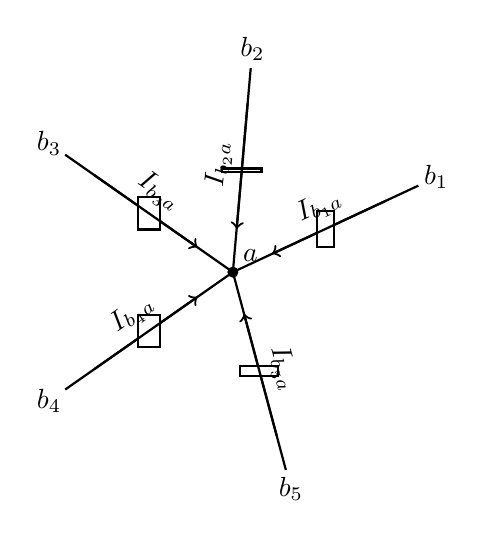
\begin{tikzpicture}[x=1cm,y=1cm,thick]
  \coordinate (a) at (0,0);
  \foreach \ang/\name/\lab in {25/b_1/I_{b_1a},85/b_2/I_{b_2a},145/b_3/I_{b_3a},215/b_4/I_{b_4a},285/b_5/I_{b_5a}} {
    \draw (a)--({2.6*cos(\ang)},{2.6*sin(\ang)});
    \draw[fill=white] ({1.3*cos(\ang)-0.25*sin(\ang)},{1.3*sin(\ang)+0.25*cos(\ang)}) rectangle
      ({1.3*cos(\ang)+0.25*sin(\ang)},{1.3*sin(\ang)-0.25*cos(\ang)});
    \draw[->] ({2.15*cos(\ang)},{2.15*sin(\ang)})--({0.55*cos(\ang)},{0.55*sin(\ang)})
      node[midway,sloped,above] {$\lab$};
    \node at ({2.85*cos(\ang)},{2.85*sin(\ang)}) {$\name$};
  }
  \fill (a) circle (2pt) node[above right] {$a$};
\end{tikzpicture}
}
 \caption{节点 \(a\) 连接若干二端支路 \(b_i a\)。各电流 \(I_{b_i a}\) 都取流入节点 \(a\) 的方向，基尔霍夫第一定律要求它们在每一时刻的代数和为零（原书图 7）。}
 \label{fig:ch2-13-kcl}
\end{figure}

图~\ref{fig:ch2-13-kcl} 表明，电流方程只涉及同一节点的各支路，不涉及节点之间的具体元件类型。若某条支路的参考方向与图中相反，只需把该电流整体变号。

若
\[
 ab,bc,\ldots,hk,ka
\]
依次构成电路中的一个闭合回路，则基尔霍夫第二定律为
\begin{equation}
 U_{ab}(t)+U_{bc}(t)+\cdots+U_{hk}(t)+U_{ka}(t)=0.
 \label{eq:ch2-13-loop-voltage}
\end{equation}

\begin{figure}[H]
 \centering
 \resizebox{0.55\textwidth}{!}{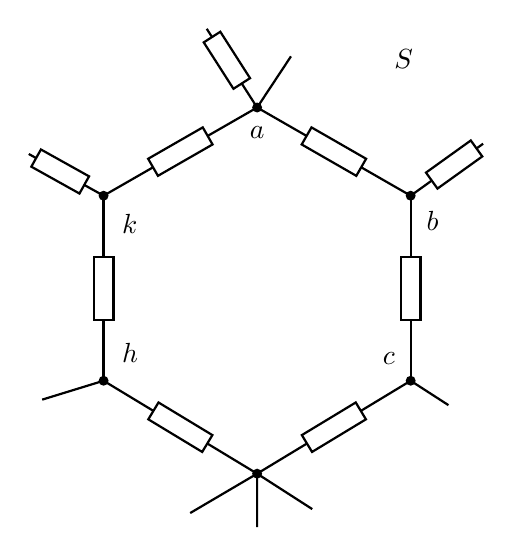
\begin{tikzpicture}[x=1cm,y=1cm,line width=0.8pt]
  \coordinate (a) at (0,2.35);
  \coordinate (b) at (1.95,1.23);
  \coordinate (c) at (1.95,-1.12);
  \coordinate (m) at (0,-2.30);
  \coordinate (h) at (-1.95,-1.12);
  \coordinate (k) at (-1.95,1.23);

  % The unlabelled lower vertex represents intermediate nodes in ab,bc,...,hk,ka.
  \foreach \from/\to in {a/b,b/c,c/m,m/h,h/k,k/a} {
    \draw (\from)--node[midway,sloped,draw,fill=white,
      minimum width=8mm,minimum height=2.5mm,inner sep=0pt]{} (\to);
  }

  % Other branches incident at the loop vertices remain visible.
  \draw (a)--++(0.43,0.65);
  \draw (a)--node[pos=0.60,sloped,draw,fill=white,
    minimum width=7mm,minimum height=2.5mm,inner sep=0pt]{} ++(-0.64,1.00);
  \draw (b)--node[pos=0.60,sloped,draw,fill=white,
    minimum width=7mm,minimum height=2.5mm,inner sep=0pt]{} ++(0.92,0.66);
  \draw (c)--++(0.48,-0.31);
  \draw (m)--++(-0.85,-0.50) (m)--++(0.70,-0.45) (m)--++(0,-0.68);
  \draw (h)--++(-0.78,-0.24);
  \draw (k)--node[pos=0.58,sloped,draw,fill=white,
    minimum width=7mm,minimum height=2.5mm,inner sep=0pt]{} ++(-0.95,0.53);

  \foreach \p in {a,b,c,m,h,k} {\fill (\p) circle (1.8pt);}
  \node[below=3pt] at (a) {$a$};
  \node[below right=2pt] at (b) {$b$};
  \node[above left=2pt] at (c) {$c$};
  \node[above right=3pt] at (h) {$h$};
  \node[below right=3pt] at (k) {$k$};
  \node at (1.86,2.96) {$S$};
\end{tikzpicture}
}
 \caption{闭合回路 \(a\to b\to c\to h\to k\to a\)。沿所有边的电压降按同一绕行方向相加，总代数和为零（原书图 8）。}
 \label{fig:ch2-13-kvl}
\end{figure}

图~\ref{fig:ch2-13-kvl} 的闭合路径说明，电压定律把沿一条闭合路径的各段电压联系起来。实际列方程时，一旦选定绕行方向，逆着绕行方向的电压就带负号；这与 \eqref{eq:ch2-13-reversed-signs} 完全一致。

若电路由 \(n\) 个二端元件组成，则共有 \(2n\) 个未知时间函数，即每个元件的电流与电压。每个元件的本构关系给出 \(n\) 个方程；基尔霍夫定律再提供 \(n\) 个彼此独立的关系。所得方程中，一部分是微分方程，一部分是有限代数方程。通常先利用基尔霍夫定律消去未知函数，再保留最小数目的独立变量代入本构关系。常见做法有两种。

\begin{enumerate}[label=\arabic*.]
 \item \textbf{回路电流法.} 取电流为基本未知函数。先利用基尔霍夫第一定律，把全部支路电流用最小数目的独立回路电流表示；再用基尔霍夫第二定律，把回路中每段电压按本构关系换成相应的电流表达式。
 \item \textbf{节点电压法.} 取电压为基本未知函数。先利用基尔霍夫第二定律，把全部电压用最小数目的独立节点电压表示；再利用基尔霍夫第一定律，把每条支路电流按本构关系换成相应的电压表达式。
\end{enumerate}

两种方法都是有限维线性代数中的基选择思想在电路中的应用：独立回路电流是电流约束的基变量，独立节点电压是电压约束的基变量。

\subsection*{二端网络的算子阻抗}

\medskip
\noindent\textbf{命题 (F)：算子阻抗与算子导纳.}
设 \(ab\) 是电阻、电感或电容。记
\begin{equation}
 U_{ab}(t)=U(t),
 \qquad
 I_{ab}(t)=I(t),
 \qquad
 R_{ab}=R,\quad L_{ab}=L,\quad C_{ab}=C.
 \label{eq:ch2-13-generic-element-data}
\end{equation}
除了前面对 \(D=d/dt\) 的记法，还自然引入
\begin{equation}
 \frac1D f(t)=\int f(t)\,\dd t.
 \label{eq:ch2-13-inverse-D}
\end{equation}
其中不定积分的常数反映电容的初始电量。在零初始条件或只研究定态时，可以把它看作普通的逆运算。

三类无源元件的本构关系可以统一写成
\begin{equation}
 U(t)=Z(D)I(t),
 \label{eq:ch2-13-impedance-law}
\end{equation}
其中
\begin{equation}
 Z_R(D)=R,
 \qquad
 Z_L(D)=LD,
 \qquad
 Z_C(D)=\frac1{CD}.
 \label{eq:ch2-13-element-impedances}
\end{equation}
函数 \(Z(D)\) 称为二端网络的\emph{算子阻抗}。电阻和电感的阻抗是 \(D\) 的多项式，电容的阻抗是有理函数。对电容方程也可写成
\begin{equation}
 U(t)=\frac1{CD}I(t),
 \label{eq:ch2-13-capacitor-impedance}
 \end{equation}
两边乘以 \(CD\) 就回到 \(I=C DU\)。

若 \(Z(D)\) 可逆，则令
\begin{equation}
 G(D)=\frac1{Z(D)},
 \label{eq:ch2-13-admittance-definition}
\end{equation}
并把 \eqref{eq:ch2-13-impedance-law} 改写成
\begin{equation}
 I(t)=G(D)U(t).
 \label{eq:ch2-13-admittance-law}
\end{equation}
\(G(D)\) 称为\emph{算子导纳}。对三种基本元件，
\[
 G_R(D)=\frac1R,
 \qquad
 G_L(D)=\frac1{LD},
 \qquad
 G_C(D)=CD.
\]

图~\ref{fig:ch2-13-terminal-impedance} 用一个方块表示二端网络只看端点时可以观察到的关系。其内部结构不必出现在端点方程中，端点行为已由算子阻抗 \(Z(D)\) 概括。

\begin{figure}[H]
 \centering
 \resizebox{0.62\textwidth}{!}{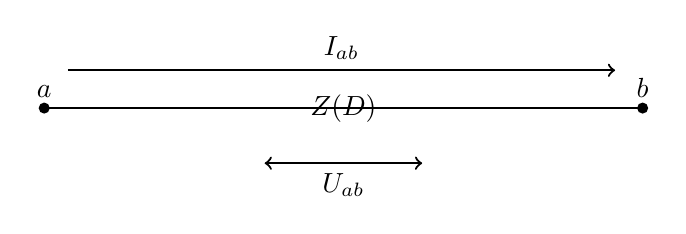
\begin{tikzpicture}[x=1cm,y=1cm,thick]
  \draw (-3.8,0)--(-1.0,0); \draw (1.0,0)--(3.8,0);
  \draw[fill=white,minimum width=2cm,minimum height=0.8cm] (-1,0) rectangle (1,0);
  \node at (0,0) {$Z(D)$};
  \fill (-3.8,0) circle (2pt) node[above] {$a$}; \fill (3.8,0) circle (2pt) node[above] {$b$};
  \draw[->] (-3.5,0.48)--(3.45,0.48) node[midway,above] {$I_{ab}$};
  \draw[<->] (-1.0,-0.7)--(1.0,-0.7) node[midway,below] {$U_{ab}$};
\end{tikzpicture}
}
 \caption{二端网络的端点模型：电流 \(I_{ab}\) 从左端 \(a\) 流向右端 \(b\)，端点电压降为 \(U_{ab}\)，端点本构关系可写成 \(U_{ab}=Z(D)I_{ab}\)（原书图 9）。}
 \label{fig:ch2-13-terminal-impedance}
\end{figure}

对互感，算子记法下的关系为
\begin{align}
 U_1(t)&=L_1D I_1(t)+MD I_2(t),
 \label{eq:ch2-13-mutual-operator-first}\\
 U_2(t)&=L_2D I_2(t)+MD I_1(t).
 \label{eq:ch2-13-mutual-operator-second}
\end{align}

实际的电路常用图表示：用点表示节点，用线段或曲线表示二端元件，在线上标记元件的约定符号。

\begin{figure}[H]
 \centering
 \resizebox{0.42\textwidth}{!}{\begin{tikzpicture}[x=1cm,y=1cm,line width=0.8pt]
  % Resistor.
  \draw (0,7.40)--(0.55,7.40) (2.00,7.40)--(2.55,7.40);
  \draw (0.55,7.25) rectangle (2.00,7.55);
  \node[above=2pt] at (1.28,7.55) {$R$};
  \node[right] at (2.95,7.40) {电阻};

  % The inductor is a sequence of upper semicircles.
  \draw (0,6.43)--(0.38,6.43);
  \draw (0.38,6.43)
    arc[start angle=180,end angle=0,radius=0.18]
    arc[start angle=180,end angle=0,radius=0.18]
    arc[start angle=180,end angle=0,radius=0.18]
    arc[start angle=180,end angle=0,radius=0.18]
    arc[start angle=180,end angle=0,radius=0.18]
    --(2.55,6.43);
  \node[above=2pt] at (1.28,6.61) {$L$};
  \node[right] at (2.95,6.43) {电感};

  % Two separate vertical windings and the coupling arch.
  \draw (0.88,5.69)--(0.88,5.49)
    arc[start angle=90,end angle=270,radius=0.14]
    arc[start angle=90,end angle=270,radius=0.14]
    arc[start angle=90,end angle=270,radius=0.14]
    arc[start angle=90,end angle=270,radius=0.14]
    --(0.88,4.15);
  \draw (1.90,5.69)--(1.90,5.49)
    arc[start angle=90,end angle=-90,radius=0.14]
    arc[start angle=90,end angle=-90,radius=0.14]
    arc[start angle=90,end angle=-90,radius=0.14]
    arc[start angle=90,end angle=-90,radius=0.14]
    --(1.90,4.15);
  \draw (1.05,5.60)..controls (1.25,5.76) and (1.53,5.76)..(1.73,5.60);
  \node[left=4pt] at (0.74,4.91) {$L_1$};
  \node[right=4pt] at (2.04,4.91) {$L_2$};
  \node[right] at (2.95,4.91) {互感};

  % Capacitor plates are separated by a genuine gap.
  \draw (0,3.67)--(1.05,3.67) (1.35,3.67)--(2.55,3.67);
  \draw[line width=2pt] (1.05,3.36)--(1.05,3.98)
    (1.35,3.36)--(1.35,3.98);
  \node[above right=1pt] at (1.35,3.85) {$C$};
  \node[right] at (2.95,3.67) {电容};

  % Source conventions in the original: negative left, positive right.
  \draw (0,2.60)--(1.05,2.60) (1.38,2.60)--(2.55,2.60);
  \draw (1.05,2.42)--(1.05,2.78) (1.38,2.24)--(1.38,2.96);
  \node[above=1pt] at (0.86,2.78) {$-$};
  \node[above=1pt] at (1.67,2.78) {$+$};

  \draw (0,1.65)--(0.84,1.65) (1.66,1.65)--(2.55,1.65);
  \fill (0.84,1.65) circle (2.4pt);
  \fill (1.66,1.65) circle (2.4pt);
  \node at (1.25,1.65) {$\sim$};

  \draw (0,0.60)--(0.84,0.60) (1.70,0.60)--(2.55,0.60);
  \draw (1.27,0.60) circle (0.43);
  \node at (1.27,0.60) {$U(t)$};
  \node[above=1pt] at (0.63,0.83) {$-$};
  \node[above=1pt] at (1.91,0.83) {$+$};

  % Hand-drawn brace; this figure needs no additional TikZ library.
  \draw (2.72,3.06)..controls (2.93,3.06) and (2.94,2.84)..(2.94,2.61)
    --(2.94,2.09)..controls (2.94,1.88) and (3.02,1.83)..(3.13,1.78)
    ..controls (3.02,1.73) and (2.94,1.68)..(2.94,1.47)
    --(2.94,0.77)..controls (2.94,0.49) and (2.91,0.19)..(2.72,0.19);
  \node[right,align=left] at (3.24,1.78) {不变的、简谐的和\\任意变动的电压源};
\end{tikzpicture}
}
 \caption{电路元件的约定记号：电阻、电感、互感、电容，以及不变、简谐和任意变动的电压源。符号只规定元件的支路关系，不规定实际电流的正负（原书图 10）。}
 \label{fig:ch2-13-symbols}
\end{figure}

图~\ref{fig:ch2-13-symbols} 中的符号用于下面三个例子。图形本身不是方程；列方程时仍须结合箭头、正负号和所选绕行方向。

\subsection*{例题 1：振荡回路}

设电路 \(S\) 有四个节点 \(a,b,c,d\)，由四个二端元件
\[
 ab,\quad bc,\quad cd,\quad da
\]
组成。元件 \(ab\) 是电感 \(L\)，\(bc\) 是电阻 \(R\)，\(cd\) 是电容 \(C\)，\(da\) 是电压源 \(U_{da}(t)=-U(t)\)，等价地 \(U_{ad}(t)=U(t)\)。

\begin{figure}[H]
 \centering
 \resizebox{0.48\textwidth}{!}{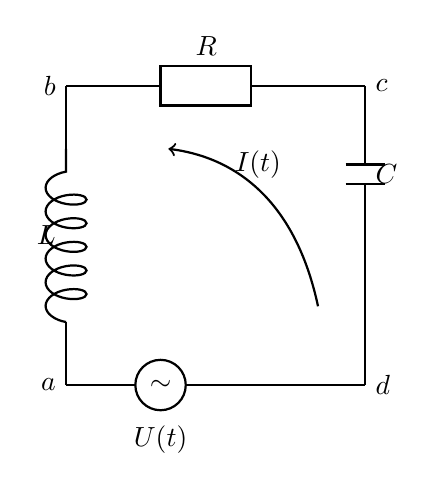
\begin{tikzpicture}[x=1cm,y=1cm,thick]
  \draw (0,0)--(0,0.8); \draw[decorate,decoration={coil,segment length=3mm,amplitude=2.6mm}] (0,0.8)--(0,3.0); \draw (0,3.0)--(0,3.8);
  \draw (0,3.8)--(1.2,3.8); \draw[fill=white] (1.2,3.55) rectangle (2.35,4.05); \node[above] at (1.78,4.05) {$R$}; \draw (2.35,3.8)--(3.8,3.8);
  \draw (3.8,3.8)--(3.8,2.8); \draw (3.55,2.8)--(4.05,2.8); \draw (3.55,2.55)--(4.05,2.55); \draw (3.8,2.55)--(3.8,0);
  \draw (0,0)--(0.88,0); \draw (1.2,0) circle (0.32); \draw (1.52,0)--(3.8,0);
  \node at (1.2,0) {$\sim$};
  \node[left] at (0,0) {$a$}; \node[left] at (0,3.8) {$b$}; \node[right] at (3.8,3.8) {$c$}; \node[right] at (3.8,0) {$d$};
  \node[left] at (0,1.9) {$L$}; \node[right] at (3.8,2.68) {$C$}; \node[below] at (1.2,-0.38) {$U(t)$};
  \draw[->] (3.2,1.0) .. controls (2.9,2.4) and (2.1,2.9) .. (1.3,3.0) node[midway,above] {$I(t)$};
\end{tikzpicture}
}
 \caption{由电感 \(L\)、电阻 \(R\)、电容 \(C\) 和电压源 \(U(t)\) 串联组成的回路；回路中只有一条独立电流，记为 \(I(t)\)（原书图 11）。}
 \label{fig:ch2-13-oscillator-circuit}
\end{figure}

采用回路电流法。在节点 \(b\) 应用基尔霍夫第一定律，有
\begin{equation}
 I_{ab}(t)+I_{cb}(t)=0;
\end{equation}
按参考方向写成常用形式就是 \(I_{ab}(t)=I_{bc}(t)\)。在只有两个二端元件相接的节点处都会得到这类等式。于是四个元件中的电流都相同，记为回路电流 \(I(t)\)：
\begin{equation}
 I_{ab}(t)=I_{bc}(t)=I_{cd}(t)=I_{da}(t)=I(t).
 \label{eq:ch2-13-loop-current}
\end{equation}

对四个元件应用本构关系：
\begin{equation}
 \left\{
 \begin{aligned}
  U_{ab}(t)&=LDI(t),\\
  U_{bc}(t)&=RI(t),\\
  U_{cd}(t)&=\frac1{CD}I(t),\\
  U_{da}(t)&=-U(t).
 \end{aligned}
 \right.
 \label{eq:ch2-13-oscillator-element-voltages}
\end{equation}
沿整个回路应用基尔霍夫第二定律：
\begin{equation}
 U_{ab}(t)+U_{bc}(t)+U_{cd}(t)+U_{da}(t)=0.
 \label{eq:ch2-13-oscillator-kvl}
\end{equation}
代入上面各式，得
\begin{equation}
 \left(LD+R+\frac1{CD}\right)I(t)=U(t).
 \label{eq:ch2-13-oscillator-impedance}
\end{equation}
这是用算子阻抗写出的串联回路方程。两边乘以 \(D\)，就得到不含逆算子的微分方程
\begin{equation}
 \left(LD^2+RD+\frac1C\right)I(t)=DU(t).
 \label{eq:ch2-13-oscillator-differential}
\end{equation}

如果从回路中除去有源元件 \(da\)，就得到断开的无源电路，它由 \(ab,bc,cd\) 三个二端元件串联组成，回路端点 \(a,d\) 之间可整体看成一个二端网络。

\begin{figure}[H]
 \centering
 \resizebox{0.56\textwidth}{!}{\begin{tikzpicture}[x=1cm,y=1cm,thick]
  \draw (0,0)--(0.8,0); \draw[decorate,decoration={coil,segment length=2.8mm,amplitude=2.3mm}] (0.8,0)--(2.1,0); \draw (2.1,0)--(2.3,0);
  \draw (2.3,-0.22) rectangle (3.25,0.22); \node at (2.78,0) {$R$}; \draw (3.25,0)--(3.5,0);
  \draw (3.5,-0.28)--(3.5,0.28); \draw (3.75,-0.28)--(3.75,0.28); \draw (3.75,0)--(4.5,0);
  \fill (0,0) circle (2pt) node[above] {$b$}; \fill (4.5,0) circle (2pt) node[above] {$a$};
  \node[below] at (1.45,-0.05) {$L$}; \node[below] at (3.62,-0.32) {$C$};
  \draw[dashed] (0,-0.72) rectangle (4.5,0.72);
  \node at (2.35,-1.3) {$Z(D)=LD+R+\dfrac{1}{CD}$};
\end{tikzpicture}
}
 \caption{从原回路中移去电压源后，电感、电阻、电容串联形成一个二端网络；其总算子阻抗为 \(Z(D)=LD+R+\frac1{CD}\)（原书图 12）。}
 \label{fig:ch2-13-disconnected-circuit}
\end{figure}

图~\ref{fig:ch2-13-disconnected-circuit} 的端点模型满足
\begin{equation}
 U_{ad}(t)=Z(D)I(t),
 \qquad
 Z(D)=LD+R+\frac1{CD}.
 \label{eq:ch2-13-series-impedance}
\end{equation}
相应的算子导纳为
\begin{equation}
 G(D)=\frac1{Z(D)}
 =\frac{CD}{LCD^2+RCD+1}.
 \label{eq:ch2-13-series-admittance}
\end{equation}

若电源 \(U(t)=0\)，电路由三个无源元件组成，两端点 \(a,d\) 重合。

\begin{figure}[H]
 \centering
 \resizebox{0.45\textwidth}{!}{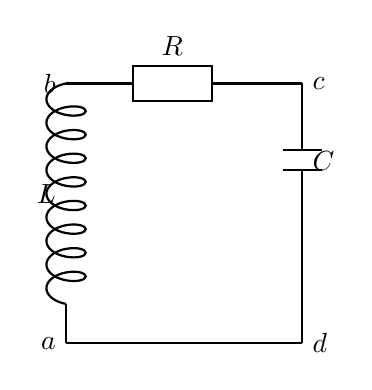
\begin{tikzpicture}[x=1cm,y=1cm,thick]
  \draw (0,0)--(0,0.5); \draw[decorate,decoration={coil,segment length=3mm,amplitude=2.5mm}] (0,0.5)--(0,3.3);
  \draw (0,3.3)--(0.85,3.3); \draw[fill=white] (0.85,3.08) rectangle (1.85,3.52); \node[above] at (1.35,3.52) {$R$}; \draw (1.85,3.3)--(3,3.3);
  \draw (3,3.3)--(3,2.45); \draw (2.75,2.45)--(3.25,2.45); \draw (2.75,2.2)--(3.25,2.2); \draw (3,2.2)--(3,0);
  \draw (0,0)--(3,0); \node[left] at (0,0) {$a$}; \node[left] at (0,3.3) {$b$}; \node[right] at (3,3.3) {$c$}; \node[right] at (3,0) {$d$};
  \node[left] at (0,1.9) {$L$}; \node[right] at (3,2.32) {$C$};
\end{tikzpicture}
}
 \caption{无源闭合振荡回路：去除电压源并以导线闭合端点后，支路中仍可存在初始电流；电感、电阻和电容共同决定其自由衰减（原书图 13）。}
 \label{fig:ch2-13-passive-loop}
\end{figure}

图~\ref{fig:ch2-13-passive-loop} 对应方程
\begin{equation}
 \left(LD^2+RD+\frac1C\right)I(t)=0.
 \label{eq:ch2-13-passive-loop-equation}
\end{equation}
无源电路不会自发产生持续电流，零函数是它的特解；但若初始时已有电流或电容已充电，仍可研究这些状态如何随时间演化。特征多项式为
\begin{equation}
 L(s)=Ls^2+Rs+\frac1C.
 \label{eq:ch2-13-loop-characteristic}
\end{equation}
因为 \(L,C>0\)，若 \(R\ge0\)，则所有系数非负且常数项为正；由 §9 命题 (B)，在 \(R>0\) 时它稳定，电流按指数速度衰减。若 \(R=0\)，则为下一段的无阻尼理想情形。

为区分衰减方式，计算判别式
\begin{equation}
 \Delta=\left(\frac{R}{2L}\right)^2-\frac1{LC}.
 \label{eq:ch2-13-loop-discriminant}
\end{equation}
若 \(\Delta<0\)，两个特征根为共轭复数，非零解具有振动特性；若 \(\Delta>0\)，两个根都是负实数，非周期地衰减。\(\Delta=0\) 是退化边界，此时有负二重根
\[
 \lambda=-\frac{R}{2L},
\]
解含因子 \(1,t\)，仍不振荡且当 \(t\to+\infty\) 时趋于零。无论 \(\Delta\) 属于哪一种，只有 \(\Delta<0\) 时才会在衰减包络下反复改变符号。

特别考虑完全没有电阻的振荡回路。此时电路只剩电感 \(ab\) 与电容 \(cd\)，并且端点满足 \(b=c,a=d\)。

\begin{figure}[H]
 \centering
 \resizebox{0.34\textwidth}{!}{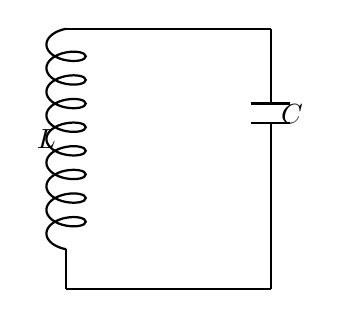
\begin{tikzpicture}[x=1cm,y=1cm,thick]
  \draw (0,0)--(0,0.5); \draw[decorate,decoration={coil,segment length=3mm,amplitude=2.5mm}] (0,0.5)--(0,3.3);
  \draw (0,3.3)--(2.6,3.3); \draw (2.6,3.3)--(2.6,2.35); \draw (2.35,2.35)--(2.85,2.35); \draw (2.35,2.1)--(2.85,2.1); \draw (2.6,2.1)--(2.6,0); \draw (0,0)--(2.6,0);
  \node[left] at (0,1.9) {$L$}; \node[right] at (2.6,2.22) {$C$};
\end{tikzpicture}
}
 \caption{无电阻的理想 LC 回路。电感与电容直接把能量相互转换，既不耗散也不产生能量，因此得到频率为 \(1/\sqrt{LC}\) 的非衰减振荡（原书图 14）。}
 \label{fig:ch2-13-lc-loop}
\end{figure}

图~\ref{fig:ch2-13-lc-loop} 的回路方程为
\begin{equation}
 \left(LD^2+\frac1C\right)I(t)=0,
 \label{eq:ch2-13-lc-equation}
\end{equation}
或
\begin{equation}
 \left(D^2+\frac1{LC}\right)I(t)=0.
 \label{eq:ch2-13-lc-normalized}
\end{equation}
通解为
\begin{equation}
 I(t)=s\cos(\omega_1t+\beta),
 \qquad
 \omega_1=\frac1{\sqrt{LC}},
 \label{eq:ch2-13-lc-solution}
\end{equation}
其中 \(s,\beta\) 是实常数。量
\[
 \omega_1=\frac1{\sqrt{LC}}
\]
称为振荡回路的固有角频率；没有电阻时，它与振幅无关，振荡永不衰减。

再回到包含简谐电压源的回路。若
\begin{equation}
 U(t)=re^{i\omega t},
 \qquad r>0,
 \label{eq:ch2-13-harmonic-loop-source}
\end{equation}
那么由 \eqref{eq:ch2-13-oscillator-differential}，
\begin{equation}
 DU(t)=ir\omega e^{i\omega t}.
 \label{eq:ch2-13-source-derivative}
\end{equation}
设定态电流为
\[
 I_{\mathrm{ss}}(t)=\sigma e^{i\omega t}.
\]
在 \eqref{eq:ch2-13-oscillator-impedance} 中取 \(D=i\omega\)，得到
\begin{align}
 \sigma
 &=\frac{ir\omega}
 {iR\omega+\left(-L\omega^2+\frac1C\right)}\notag\\
 &=\frac{r}{R+i\left(L\omega-\frac1{C\omega}\right)}.
 \label{eq:ch2-13-loop-complex-amplitude}
\end{align}
因此定态电流的实振幅为
\begin{equation}
 s=|\sigma|
 =\frac{r}
 {\sqrt{R^2+\left(L\omega-\frac1{C\omega}\right)^2}}.
 \label{eq:ch2-13-loop-amplitude}
\end{equation}
对固定振幅 \(r\) 的电源，当
\begin{equation}
 L\omega-\frac1{C\omega}=0,
 \qquad
 \omega=\frac1{\sqrt{LC}}=\omega_1
 \label{eq:ch2-13-loop-resonance}
\end{equation}
时分母最小，电流振幅达到最大值
\[
 s=\frac rR.
\]
也就是说，在共振频率处，回路表现得好似只有电阻 \(R\) 存在。对其他频率，振幅都小于 \(r/R\)。这就是 RLC 振荡回路的共振现象。

\subsection*{例题 2：变压器}

变压器由安装在同一铁芯上的原绕组和副绕组构成。原绕组接可变电压源，副绕组接负载，例如外电阻。每个绕组都有电感和内电阻；两个绕组之间还有互感。因此可把变压器看成两个通过互感耦合的回路。

\begin{figure}[H]
 \centering
 \resizebox{0.68\textwidth}{!}{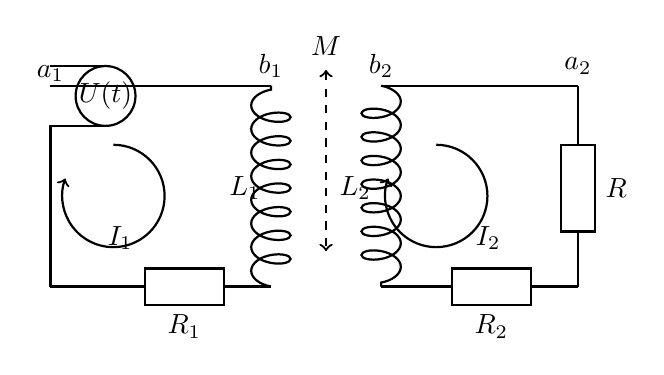
\begin{tikzpicture}[x=1cm,y=1cm,thick]
  % Coupled primary and secondary loops with distinct current arrows.
  \draw (0,0)--(0.7,0); \draw (0.7,-0.38) circle (0.38); \node at (0.7,-0.38) {$U(t)$}; \draw (0.7,-0.76)--(0,-0.76)--(0,-2.8);
  \draw (0,-2.8)--(1.2,-2.8); \draw[fill=white] (1.2,-3.03) rectangle (2.2,-2.57); \node[below] at (1.7,-3.03) {$R_1$}; \draw (2.2,-2.8)--(2.8,-2.8);
  \draw[decorate,decoration={coil,segment length=3mm,amplitude=2.5mm}] (2.8,-2.8)--(2.8,-0.25); \draw (2.8,-0.25)--(0,-0.25);
  \draw (4.2,-0.25)--(6.7,-0.25); \draw[decorate,decoration={coil,segment length=3mm,amplitude=2.5mm}] (4.2,-0.25)--(4.2,-2.8); \draw (4.2,-2.8)--(5.1,-2.8);
  \draw[fill=white] (5.1,-3.03) rectangle (6.1,-2.57); \node[below] at (5.6,-3.03) {$R_2$}; \draw (6.1,-2.8)--(6.7,-2.8);
  \draw (6.7,-2.8)--(6.7,-0.25); \draw (6.7,-1.0)--(6.7,-2.1); \draw[fill=white] (6.48,-2.1) rectangle (6.92,-1.0); \node[right] at (6.92,-1.55) {$R$};
  \node[left] at (2.8,-1.55) {$L_1$}; \node[left] at (4.2,-1.55) {$L_2$};
  \node at (3.5,0.25) {$M$}; \draw[<->,dashed] (3.5,-0.05)--(3.5,-2.35);
  \draw[->] (0.8,-1.0) arc[start angle=90,end angle=-200,radius=0.65] node[midway,left] {$I_1$};
  \draw[->] (4.9,-1.0) arc[start angle=90,end angle=-200,radius=0.65] node[midway,right] {$I_2$};
  \node at (0,-0.1) {$a_1$}; \node at (2.8,0) {$b_1$}; \node at (4.2,0) {$b_2$}; \node at (6.7,0) {$a_2$};
\end{tikzpicture}
}
 \caption{互感耦合的变压器模型：原边回路含电源 \(U(t)\)、电感 \(L_1\) 和内电阻 \(R_1\)，副边回路含电感 \(L_2\)、内电阻 \(R_2\) 与负载电阻 \(R\)，两电感以 \(M\) 耦合（原书图 15）。}
 \label{fig:ch2-13-transformer}
\end{figure}

图~\ref{fig:ch2-13-transformer} 中第一个回路有三个二端元件：电感 \(L_1\)、内电阻 \(R_1\) 和电压源 \(U(t)\)。第二个回路也有三个：电感 \(L_2\)、内电阻 \(R_2\) 和负载电阻 \(R\)。此外还有互感
\[
 M=M_{a_1b_1,a_2b_2}.
\]
设两个回路电流分别为 \(I_1,I_2\)。在每个只有两个元件相接的节点处应用基尔霍夫第一定律，可知同一绕组回路中的所有支路电流相同。于是两个回路的回路电流正是 \(I_1,I_2\)。

对两个回路应用基尔霍夫第二定律并代入互感本构关系，得到
\begin{align}
 L_1DI_1+MDI_2+R_1I_1-U(t)&=0,
 \label{eq:ch2-13-transformer-loop1}\\
 L_2DI_2+MDI_1+R_2I_2+RI_2&=0.
 \label{eq:ch2-13-transformer-loop2}
\end{align}
整理成标准形式：
\begin{align}
 (L_1D+R_1)I_1+MDI_2&=U(t),
 \label{eq:ch2-13-transformer-system1}\\
 MDI_1+(L_2D+R_2+R)I_2&=0.
 \label{eq:ch2-13-transformer-system2}
\end{align}

系数矩阵的行列式为
\begin{align}
 D_{\mat{L}}(s)
 &=(L_1s+R_1)(L_2s+R_2+R)-M^2s^2\notag\\
 &=(L_1L_2-M^2)s^2
   +\bigl(L_1(R_2+R)+R_1L_2\bigr)s
   +R_1(R_2+R).
 \label{eq:ch2-13-transformer-determinant}
\end{align}
由 \(M^2<L_1L_2\) 以及正的电阻值，三个系数都为正。它是二次实多项式，由 §9 命题 (B)，稳定；因此自由响应随时间衰减，可以讨论唯一的定态响应。

设原边电压为复简谐函数
\begin{equation}
 U(t)=u_1e^{i\omega t},
 \qquad u_1>0.
 \label{eq:ch2-13-transformer-harmonic-source}
\end{equation}
寻找
\begin{equation}
 I_1(t)=\sigma_1e^{i\omega t},
 \qquad
 I_2(t)=\sigma_2e^{i\omega t}.
 \label{eq:ch2-13-transformer-complex-currents}
\end{equation}
代入 \eqref{eq:ch2-13-transformer-system1}--\eqref{eq:ch2-13-transformer-system2}，约去 \(e^{i\omega t}\)：
\begin{align}
 (iL_1\omega+R_1)\sigma_1+iM\omega\sigma_2&=u_1,
 \label{eq:ch2-13-transformer-phasors1}\\
 iM\omega\sigma_1+(iL_2\omega+R_2+R)\sigma_2&=0.
 \label{eq:ch2-13-transformer-phasors2}
\end{align}

理论分析中最重要的是理想变压器极限：内电阻 \(R_1,R_2\) 以及漏感量 \(L_1L_2-M^2\) 都很小。忽略这些小量后，
\begin{align}
 iL_1\omega\sigma_1+iM\omega\sigma_2&=u_1,
 \label{eq:ch2-13-ideal-transformer1}\\
 iM\omega\sigma_1+(iL_2\omega+R)\sigma_2&=0.
 \label{eq:ch2-13-ideal-transformer2}
\end{align}
此时 \(M\approx\sqrt{L_1L_2}\)。把第一式乘以 \(\sqrt{L_2/L_1}\)，再减去第二式，第一组中的 \(\sigma_1\) 项因
\[
 \sqrt{\frac{L_2}{L_1}}\,L_1=\sqrt{L_1L_2}\approx M
\]
而抵消，得到
\begin{equation}
 R\sigma_2=-\sqrt{\frac{L_2}{L_1}}u_1.
 \label{eq:ch2-13-transformer-load-current}
\end{equation}
因此负载 \(R\) 上的电压振幅为
\begin{equation}
 u_2=R|\sigma_2|
 =\sqrt{\frac{L_2}{L_1}}u_1.
 \label{eq:ch2-13-transformer-voltage-ratio}
\end{equation}
比值
\[
 \sqrt{\frac{L_2}{L_1}}
\]
称为变压器的变压系数。若 \(L_2>L_1\)，则 \(u_2/u_1>1\)，这是升压变压器；若 \(L_2<L_1\)，则 \(u_2/u_1<1\)，这是降压变压器。

\subsection*{例题 3：电子滤波器}

考虑有四个节点 \(a,b,c,d\) 和五个二端元件的电路：\(ab\) 是电感 \(L\)，\(bc\) 是具有同样电感 \(L\) 的电感，\(bd\) 是电容 \(C\)，\(ad\) 是电压源 \(U_{ad}(t)=U(t)\)，\(cd\) 是负载电阻 \(R\)。

\begin{figure}[H]
 \centering
 \resizebox{0.72\textwidth}{!}{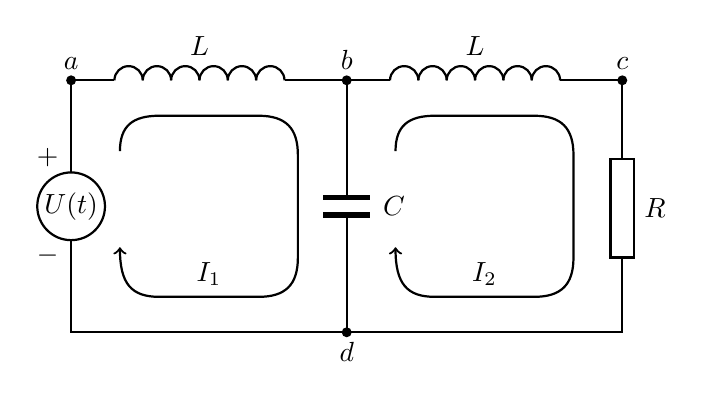
\begin{tikzpicture}[x=1cm,y=1cm,thick]
  % Two series inductors; shunt capacitor bd has a real dielectric gap.
  \draw (0,3.2)--(0.55,3.2);
  \foreach \k in {0,...,5}
    \draw ({0.55+0.36*\k},3.2) arc[start angle=180,end angle=0,radius=0.18];
  \draw (2.71,3.2)--(3.5,3.2)--(4.05,3.2);
  \foreach \k in {0,...,5}
    \draw ({4.05+0.36*\k},3.2) arc[start angle=180,end angle=0,radius=0.18];
  \draw (6.21,3.2)--(7,3.2)--(7,2.2);
  \draw (6.85,0.95) rectangle (7.15,2.2);
  \draw (7,0.95)--(7,0)--(0,0)--(0,1.17);
  \draw (0,1.6) circle (0.43);
  \draw (0,2.03)--(0,3.2);
  \node at (0,1.6) {$U(t)$};
  \node[left] at (-0.03,2.22) {$+$}; \node[left] at (-0.03,0.98) {$-$};
  \draw (3.5,3.2)--(3.5,1.71);
  \draw[line width=2pt] (3.2,1.71)--(3.8,1.71) (3.2,1.49)--(3.8,1.49);
  \draw (3.5,1.49)--(3.5,0);
  \fill (0,3.2) circle (1.8pt) node[above] {$a$};
  \fill (3.5,3.2) circle (1.8pt) node[above] {$b$};
  \fill (7,3.2) circle (1.8pt) node[above] {$c$};
  \fill (3.5,0) circle (1.8pt) node[below] {$d$};
  \node[above] at (1.63,3.38) {$L$}; \node[above] at (5.13,3.38) {$L$};
  \node[right] at (3.83,1.60) {$C$}; \node[right] at (7.15,1.575) {$R$};
  \draw[->] (0.62,2.3)
    .. controls (0.62,2.62) and (0.78,2.75) .. (1.12,2.75)
    --(2.38,2.75)
    .. controls (2.73,2.75) and (2.88,2.59) .. (2.88,2.25)
    --(2.88,0.95)
    .. controls (2.88,0.6) and (2.72,0.45) .. (2.38,0.45)
    --(1.12,0.45)
    .. controls (0.77,0.45) and (0.62,0.61) .. (0.62,1.08);
  \node[above] at (1.75,0.46) {$I_1$};
  \draw[->] (4.12,2.3)
    .. controls (4.12,2.62) and (4.28,2.75) .. (4.62,2.75)
    --(5.88,2.75)
    .. controls (6.23,2.75) and (6.38,2.59) .. (6.38,2.25)
    --(6.38,0.95)
    .. controls (6.38,0.6) and (6.22,0.45) .. (5.88,0.45)
    --(4.62,0.45)
    .. controls (4.27,0.45) and (4.12,0.61) .. (4.12,1.08);
  \node[above] at (5.25,0.46) {$I_2$};
\end{tikzpicture}
}
 \caption{两级 LC 低通滤波器：两个等值电感 \(L\) 分处上支路，电容 \(C\) 跨接在中间节点 \(b\) 与下节点 \(d\) 之间，负载电阻 \(R\) 接在右端；回路电流分别为 \(I_1,I_2\)（原书图 16）。}
 \label{fig:ch2-13-filter}
\end{figure}

图~\ref{fig:ch2-13-filter} 中用两个回路电流 \(I_1,I_2\) 表示支路电流：
\begin{equation}
 I_{ab}=I_1,
 \qquad
 I_{bc}=I_2.
 \label{eq:ch2-13-filter-loop-currents}
\end{equation}
在节点 \(b\) 应用基尔霍夫第一定律，得到
\begin{equation}
 I_{bd}=I_1-I_2,
 \qquad
 I_{cd}=I_2.
 \label{eq:ch2-13-filter-branch-currents}
\end{equation}

沿左侧大回路和右侧回路分别应用基尔霍夫第二定律：
\begin{align}
 U_{ab}+U_{bc}+U_{cd}+U_{da}&=0,
 \label{eq:ch2-13-filter-kvl1}\\
 U_{bc}+U_{cd}+U_{db}&=0.
 \label{eq:ch2-13-filter-kvl2}
\end{align}
代入本构关系：
\begin{align}
 LDI_1+LDI_2+RI_2-U(t)&=0,
 \label{eq:ch2-13-filter-equations1}\\
 LDI_2+RI_2+\frac1{CD}(I_2-I_1)&=0.
 \label{eq:ch2-13-filter-equations2}
\end{align}
把第二式乘以 \(D\)，整理为
\begin{align}
 LDI_1+(LD+R)I_2&=U(t),
 \label{eq:ch2-13-filter-system1}\\
 -\frac1C I_1+\left(LD^2+RD+\frac1C\right)I_2&=0.
 \label{eq:ch2-13-filter-system2}
\end{align}

系数矩阵的行列式为
\begin{equation}
 D_{\mat{L}}(s)
 =L^2s^3+LRs^2+\frac{2L}{C}s+\frac{R}{C}.
 \label{eq:ch2-13-filter-determinant}
\end{equation}
它的首项系数为正，所有系数都为正，并且
\[
 (LR)\left(\frac{2L}{C}\right)
 > L^2\left(\frac{R}{C}\right).
\]
由定理 6，三次多项式 \(D_{\mat{L}}(s)\) 稳定。因此滤波器存在稳定定态。

研究复简谐输入
\begin{equation}
 U(t)=be^{i\omega t},
 \qquad b>0,
 \label{eq:ch2-13-filter-input}
\end{equation}
并设
\begin{equation}
 I_1(t)=\alpha_1e^{i\omega t},
 \qquad
 I_2(t)=\alpha_2e^{i\omega t}.
 \label{eq:ch2-13-filter-complex-currents}
\end{equation}
在 \eqref{eq:ch2-13-filter-system1}--\eqref{eq:ch2-13-filter-system2} 中取 \(D=i\omega\)，可先由第二式得到
\begin{equation}
 \alpha_1
 =C\left(-L\omega^2+iR\omega+\frac1C\right)\alpha_2.
 \label{eq:ch2-13-filter-alpha1}
\end{equation}
再代回第一式并解出
\begin{equation}
 \alpha_2=
 \frac{b/C}
 {\left(\frac RC-LR\omega^2\right)
  +i\omega\left(\frac{2L}{C}-L^2\omega^2\right)}.
 \label{eq:ch2-13-filter-alpha2}
\end{equation}

负载电阻上的电压降为 \(U_{cd}=RI_2\)，其振幅为
\begin{equation}
 a=|\alpha_2|R
 =\frac{bR/C}
 {\sqrt{\left(\frac RC-LR\omega^2\right)^2
 +\omega^2\left(\frac{2L}{C}-L^2\omega^2\right)^2}}.
 \label{eq:ch2-13-filter-output-amplitude}
\end{equation}
因此
\begin{equation}
 \frac ab
 =\frac{R/C}
 {\sqrt{\left(\frac RC-LR\omega^2\right)^2
 +\omega^2\left(\frac{2L}{C}-L^2\omega^2\right)^2}}.
 \label{eq:ch2-13-filter-transfer}
\end{equation}

当频率 \(\omega\) 很小时，分母近似为 \(R/C\)，所以
\[
 \frac ab\approx1.
\]
低频电压几乎原样传到负载。当频率很大时，分母主项由
\(LR\omega^2\) 与 \(L^2\omega^3/C\) 给出，其中三次项占主导，因而
\begin{equation}
 \frac ab\approx\frac{R}{CL^2\omega^3}.
 \label{eq:ch2-13-filter-high-frequency}
\end{equation}
比值迅速趋近于零，高频信号几乎不能通过。于是这个电路表现为低通滤波器：低频容易通过，高频被“滤掉”。这里的“稳定”“定态”“滤掉”都是对上述理想线性模型而言；真实滤波器还受元件寄生效应、负载变化和物理功率限制的影响。
